\documentclass{beamer}
\RequirePackage{luatex85}
\include{../style/cours-style.sty}

% Title
\title{Scripting - Bachelor CSI}
\author{Christophe Brun}
\institute{Campus Saint-Michel IT}
\date{25 juin 2024}
\beamertemplatenavigationsymbolsempty

\titlegraphic{
    \bigbreak
    
\includegraphics[width=2cm]{image/logo-papit}
    
\includegraphics[width=2cm]{image/logo-campus-saint-michel-it}
}
\begin{document}

    \begin{frame}
        \titlepage
        \bigbreak
        \centering
        \url{https://github.com/St-Michel-IT/scripting/}
    \end{frame}

    \begin{frame}{Table des matières}
        \tableofcontents
    \end{frame}


    \section{Programme du module}\label{sec:programme-du-module}
    \begin{frame}{Scripting}{Programme et compétence}
        \begin{itemize}
            \item Chapitre 1 : Introduction à l'automatisation et au Scripting système
            \begin{itemize}
                \item Comprendre les principes de l'automatisation des tâches d'administration
                \item Identifier les avantages de l'automatisation en termes d'efficacité opérationnelle
                \item Présenter les langages de Scripting (Python, Shell, Bash) et leurs domaines d'application
                \item Expliquer l'importance de l'automatisation dans la réduction des délais de réponse en cas de problèmes ou de maintenance
                \item Définir les bonnes pratiques en matière d'automatisation et de Scripting
            \end{itemize}
        \end{itemize}
        Compétence~:
        \bigbreak
        Automatiser les tâches d'administration en développant et en appliquant des scripts en Python, Shell, et Bash, pour augmenter l'efficacité opérationnelle et réduire les délais de réponse en cas de problèmes ou de besoins de maintenance.
    \end{frame}


    \begin{frame}{Intervenant sur le module Scripting}{Christophe Brun, conseil en développement informatique}

        \begin{columns}
            \column{0.7\textwidth}
            \begin{itemize}
                \item 2\textsuperscript{nde} année d'intervenant à Saint-Michel \emoji{star-struck}.

                \item 7 ans de conseil en développement au sein d'SSII~.

                \item 8 ans de conseil en développement à mon compte \href{https://papit.fr}{PapIT}.

                \item Passionné~!
                \bigbreak
                \begin{columns}
                    \column{0.5\textwidth}
                    \centering
                    
\includegraphics[width=3cm]{image/logo-uppa}
                    \column{0.5\textwidth}
                    \centering
                    
\includegraphics[width=3cm]{image/logo-universite-bordeaux}
                \end{columns}
            \end{itemize}
            \column{0.3\textwidth}
            \centering
            
\includegraphics[width=5cm]{image/trombine-christophe}
        \end{columns}
    \end{frame}


    \section{Shell et commandes de base}\label{sec:shell-and-command}

    \subsection{Shell}\label{subsec:shell}

    \begin{frame}{Shell}{Qu'est-ce~?}
        Shell c'est~:
        \begin{itemize}
            \item C'est un exécutable.
            \item Un interpréteur de ligne de commande.
            Ne pas confondre avec des Shells spécifiques comme le Python Shell ou le MySQL Shell qui interagissent spécifiquement avec ces applications.
            \item Et donc un interpréteur de scripts Shell.
            \item C'est une interface entre l'OS et l'humain.
            \item Existe sur la plupart des plateformes Linux, Unix, Windows® (\lstinline{Bash}, installé avec Git par exemple), \textit{etc}.
            \item Une portabilité poussée par une standardisation, comme la standardisation POSIX~.
            \item Des Shells plus \textit{user friendly} et plus lourds comme \lstinline{zsh}.
            \item Des Shells éxotiques comme \lstinline{tcsh} et \lstinline{csh}.
        \end{itemize}
    \end{frame}

    \begin{frame}{Shell}{Bourne Shell VS Bourne Again Shell\footnote{Difference between sh and bash, \url{https://www.geeksforgeeks.org/difference-between-sh-and-bash/}}}
        \begin{footnotesize}
            \begin{table}[h!]
                \centering
                \begin{tabular}{|p{5.5cm}|p{5.5cm}|}
                    \hline
                    \textbf{bash}                                     & \textbf{sh}                               \\ \hline
                    Bourne Again SHell                                & SHell                                     \\ \hline
                    Developed by Brain Fox                            & Developed by Stephen R. Bourne            \\ \hline
                    Successor of sh                                   & Predecessor of bash                       \\ \hline
                    bash is the default SHELL                         & sh is not the default SHELL               \\ \hline
                    \lstinline{\#\!/bin/bash}                         & \lstinline{\#\!/bin/sh}                   \\ \hline
                    It has more functionality with up-gradation       & It has less functionality                 \\ \hline
                    Supports job controls                             & Does not support job control              \\ \hline
                    bash is not a valid POSIX shell                   & POSIX compliant, more portable            \\ \hline
                    Easy to use                                       & Not as easy as Bash                       \\ \hline
                    Extended version of language                      & Original language                         \\ \hline
                    Bash scripting is scripting specifically for Bash & Shell scripting is scripting in any shell \\ \hline
                    Supports command history                          & Does not support command history          \\ \hline
                    Associative arrays                                & Does not support associative arrays       \\ \hline
                \end{tabular}
            \end{table}
        \end{footnotesize}
    \end{frame}

    \begin{frame}[fragile]{Shell}{Qu'est-ce~?}
        2 Shells sous une même distribution \textquote{légère} comme Alpine Linux~:
        \begin{lstlisting}[language=bash]
root@71641013d445:/usr/src/celia# sh
# ls
 Dockerfile       README.pdf         UML-Sequence.drawio       celia.ipynb
# which sh
/usr/bin/sh
# which ls
/usr/bin/ls
# bash
root@71641013d445:/usr/src/celia# which bash
/usr/bin/bash
root@71641013d445:/usr/src/celia# which ls
/usr/bin/ls
root@71641013d445:/usr/src/celia# ls
 Dockerfile       README.pdf         UML-Sequence.drawio       celia.ipynb
        \end{lstlisting}
        \bigbreak
        Comment interpréter ce code~?
    \end{frame}

    \begin{frame}{Shell}{Bourne Shell VS Bourne Again Shell}
        Peut-on lister les avantages/inconvénients de l'un et l'autre~?
        \bigbreak
        \centering
        
\includegraphics[width=3cm]{image/question-mark-on-a-blank-background.png}
    \end{frame}

    \begin{frame}{Shell}{Le poid de cette interface\footnote{Exigences matérielles pour utiliser Ubuntu, \url{https://doc.ubuntu-fr.org/exigences_minimales}}}
        Minimum 30 Go d'espace disque disponible pour une installation avec GNOME contre 5 Go ou 6 Go pour une installation Server ou Cloud.
        \bigbreak
        L'absence de bureau, avoir uniquement cette interface, est une des raisons de cette différence de taille.

        L'interface graphique n'est donc pas installée dans les distributions dédiées aux serveurs.
        Shell et l'accès Shell distant sécurisé SSH (Secure SHell), sont utilisés.
        Un client SSH comme Putty, SSH de GitBASH sous Windows® ou un terminal sous Linux permettent d'accéder à un server Linux.
        \bigbreak
        GitBash permet d'unifier les deux environnements Linux et Windows, de pratiquer le Bash sur les 2 plateformes.
    \end{frame}

    \begin{frame}{Shell}{Pourquoi a-t-on un Shell ou l'autre~?}
        Quand je me connecte avec mon utilisateur, j'ai souvent \lstinline{bash} comme Shell.
        Pourquoi pas \lstinline{sh}~?
        \bigbreak
        \centering
        
\includegraphics[width=3cm]{image/question-mark-on-a-blank-background.png}
    \end{frame}

    \begin{frame}[fragile]{Shell}{Pourquoi a-t-on un Shell ou l'autre~?}
        Probablement, l'administrateur système a créé votre utilisateur en spécifiant \lstinline{bash} comme Shell.
        \bigbreak
        Si on lit l'aide de la commande \lstinline{useradd}~:
        \begin{lstlisting}[language=bash]
$ useradd -h | grep shell
  -s, --shell SHELL               interpréteur de commandes de connexion du nouveau compte
        \end{lstlisting}
        \bigbreak
        Un exemple de commande devient donc~:
        \begin{lstlisting}[language=bash]
$ useradd -s /bin/bash -m -d /home/digiformateur digicomp
        \end{lstlisting}
        \bigbreak
        \lstinline{/bin/bash} passé à l'option \lstinline{-s} permet de spécifier le Shell.
    \end{frame}

    \begin{frame}{Shell}{Naviguer dans les commandes}
        \begin{itemize}
            \item \lstinline{history}~: Affiche l'historique des commandes.
            \item Ctrl+c~: Arrête l'exécution d'une commande.
            \item \emoji{up-arrow}~: Rappelle la dernière commande.
            \item \emoji{down-arrow}~: Rappelle la commande suivante.
            \item Ctrl+r~: Recherche dans l'historique des commandes.
            \item \lstinline{\\}~: Permet de continuer une commande sur la ligne d'après.
            \item \lstinline{\&}~: Lancer une commande en arrière-plan.
            \item Ctrl+z~: Mettre une commande en pause.
            \item \lstinline{fg}~: Reprendre une commande en pause.
            \item \lstinline{bg}~: Reprendre une commande en pause en arrière-plan.
        \end{itemize}
    \end{frame}

    \begin{frame}{Shell}{Gérer plusieurs commandes en parallèle avec \lstinline{tmux}\footnote{\label{tmux}Tmux (terminal multiplexer), \url{https://www.redhat.com/sysadmin/introduction-tmux-linux}}}
        \lstinline{tmux} est un multiplexeur de terminal, \textit{i.e.}, permet d'ouvrir plusieurs fenêtres dans un terminal.
        Chacune faisant tourner un processus.
        \begin{footnotesize}
            \begin{table}[ht]
                \centering
                \begin{tabular}{|p{3.5cm}|p{8cm}|}
                    \hline
                    \textbf{Commande}                                     & \textbf{Description}                                                            \\
                    \hline
                    Ctrl+b puis D                                         & Détacher de la session courante                                                 \\
                    \hline
                    Ctrl+b puis \%                                        & Diviser la fenêtre en deux volets horizontalement                               \\
                    \hline
                    Ctrl+b puis ``                                        & Diviser la fenêtre en deux volets verticalement                                 \\
                    \hline
                    Ctrl+b puis \emoji{left-arrow} ou \emoji{right-arrow} & Se déplacer entre les volets                                                    \\
                    \hline
                    Ctrl+b puis X                                         & Fermer le volet                                                                 \\
                    \hline
                    Ctrl+b puis C                                         & Créer une nouvelle fenêtre                                                      \\
                    \hline
                    Ctrl+b puis N ou P                                    & Passer à la fenêtre suivante ou précédente                                      \\
                    \hline
                    Ctrl+b puis 0 (1,2\ldots)                             & Aller à une fenêtre spécifique par numéro                                       \\
                    \hline
                    Ctrl+b puis~:                                         & Entrer dans la ligne de commande pour taper des commandes (avec autocomplétion) \\
                    \hline
                    Ctrl+b puis ?                                         & Voir tous les raccourcis clavier (appuyer sur Q pour quitter)                   \\
                    \hline
                    Ctrl+b puis W                                         & Ouvrir un panneau pour naviguer entre les fenêtres de plusieurs sessions        \\
                    \hline
                \end{tabular}
            \end{table}
        \end{footnotesize}
    \end{frame}

    \begin{frame}{Shell}{Gérer plusieurs commandes en parallèle avec \lstinline{tmux}\cref{tmux}}
        Par exemple pour monitorer les ressources avec \lstinline{top} dans le terminal de droite, pendant qu'on lance la commande dans celui de gauche.
        \bigbreak
        \centering
        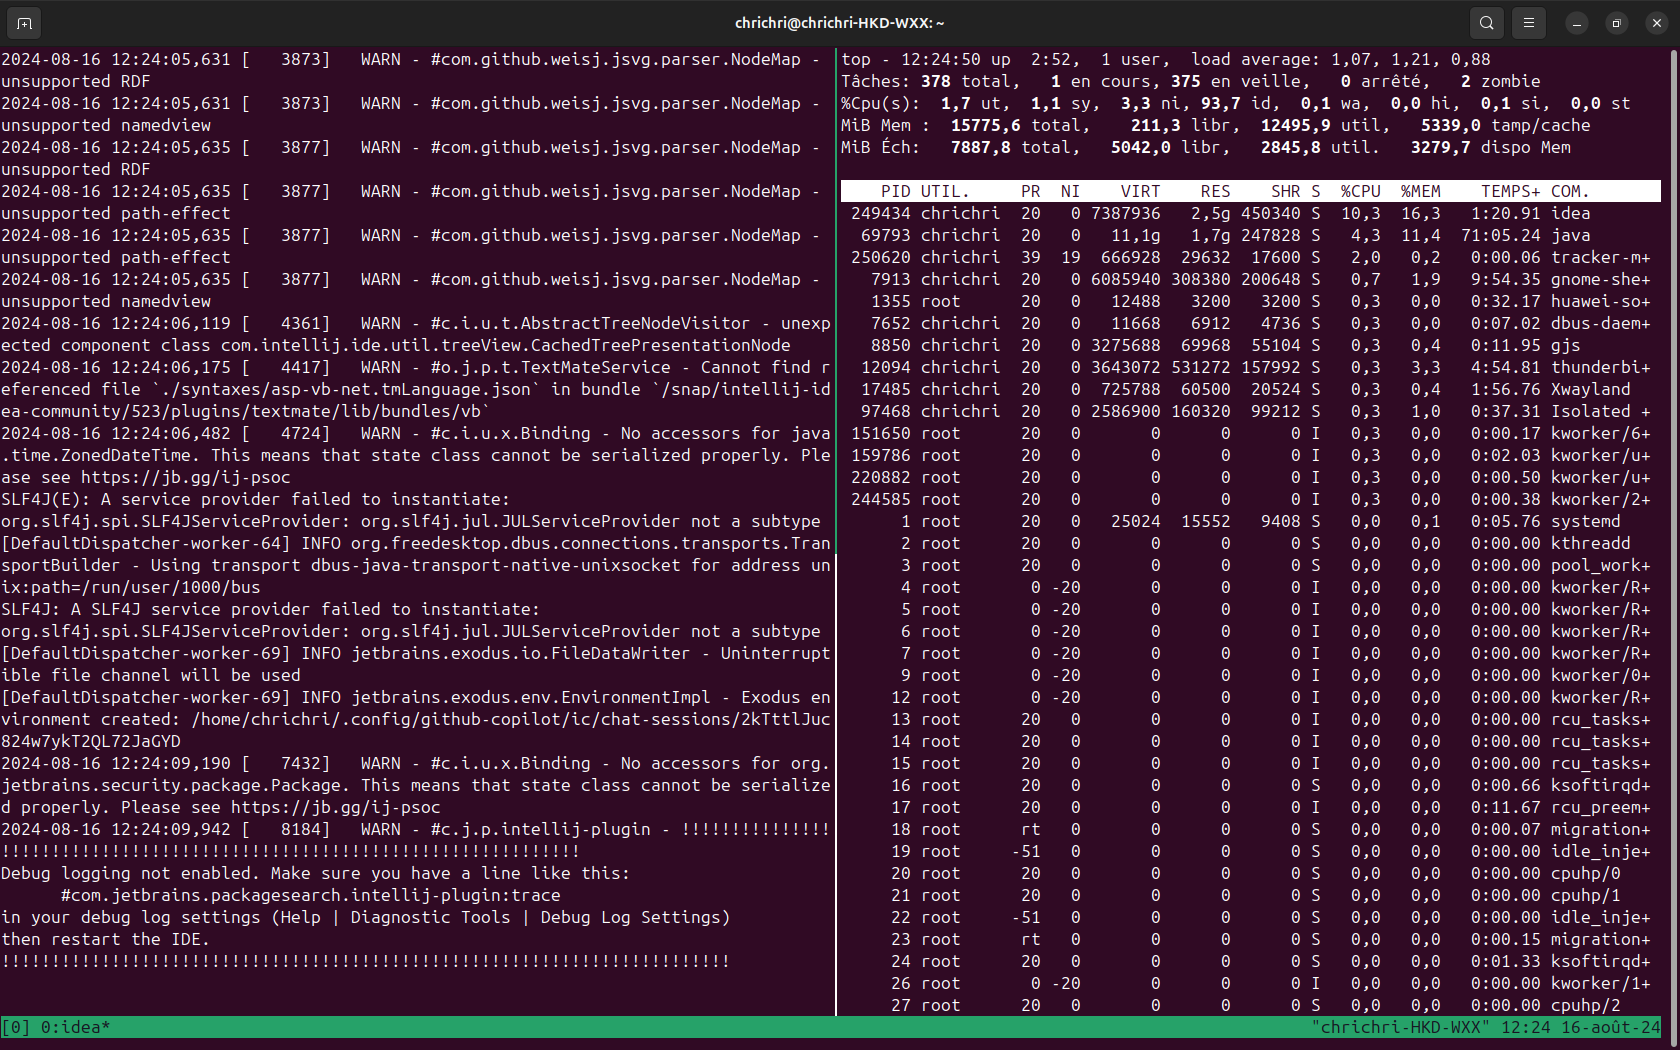
\includegraphics[width=10.3cm]{image/tmux-illustration}
    \end{frame}

    \begin{frame}[fragile]{Shell}{Gérer plusieurs commandes en parallèle avec \lstinline{nohup}}
        \lstinline{nohup} vient de NO Hang UP, c'est une commande qui permet de lancer une autre commande en arrière-plan sans qu'elle soit interrompue par la fermeture de la session Shell.
        Idéale donc pour les longs processus.
        L'output de la commande va par défault dans le fichier \lstinline{nohup.out}.
        \bigbreak
        Il suffit de préfixer la commande par \lstinline{nohup} et d'ajouter un \lstinline{&} pour libérer le terminal.
        \lstinline{nohup} indique le PID pour pouvoir stopper la commande au besoin et indique également quand la commande est terminée, si elle s'est arrêtée (Termine <code retour>) prématurément ou normalement (Fini).
        \begin{lstlisting}[language=bash]
$ nohup ls &
[1] 279343
nohup: les entrées sont ignorées et la sortie est ajoutée à 'nohup.out'
[1]+  Fini                    nohup ls
$ tail -n 3 nohup.out
technip
Téléchargements
ts-test
        \end{lstlisting}
    \end{frame}

    \begin{frame}[fragile]{Shell}{Les alias}
        Les alias sont des raccourcis pour des commandes.
        ils sont donc intéressant à paramétrer pour les commandes longues et récurrentes.
        \bigbreak
        Par exemple, pour la commande \lstinline{ls -l}~:
        \begin{lstlisting}[language=bash]
$ alias ll='ls -l'
$ ll
total 3484
-rw-rw-r-- 1 chrichri chrichri     249 août  15 12:35 analytic-using-awk.sh
-rw-rw-r-- 1 chrichri chrichri      82 août  10 23:04 checkmytex.sh
...
        \end{lstlisting}
        \bigbreak
        Pour rendre l'alias permanent, il faut l'ajouter dans le fichier \lstinline{.bashrc} ou \lstinline{.bash_profile}~:
        \begin{lstlisting}[language=bash]
$ echo "alias ll='ls -l'" >> ~/.bashrc
        \end{lstlisting}
        De cette manière à chaque fois qu'un Shell est ouvert, la commande est exécutée.
    \end{frame}

    \begin{frame}{Shell}{Secure SHell (SSH)}
        La machine Linux à administrer sera le plus souvent dans un cloud, une salle serveur, un data center, elle sera distante.
        Dans une infrastructure sécurisée.
        \bigbreak
        Mais avec un user, un Shell par défaut, et un protocole sécurisé comme le SSH, nous allons pouvoir nous connecter et l'administrer à distance.
        \bigbreak
        Les bonnes pratiques sont d'utiliser les clés SSH uniquement, pas de connexion SSH avec l'utilisateur root,
        tutoriel utile~:
        \begin{itemize}
            \item \href{https://phoenixnap.com/kb/generate-setup-ssh-key-ubuntu}{Configuration du login SSH sur Ubuntu}
        \end{itemize}
        \bigbreak
        \centering
        
\includegraphics[width=3cm]{image/student-in-front-of-desktop}
    \end{frame}

    \subsection{Commandes de base}\label{subsec:commandes-de-base}

    \begin{frame}{Commandes de base}{Commandes de base}
        \begin{itemize}
            \item \lstinline{ls}~: Liste les fichiers et répertoires.
            \item \lstinline{cd}~: Change de répertoire.
            \item \lstinline{pwd}~: Affiche le répertoire courant.
            \item \lstinline{cp}~: Copie des fichiers et des répertoires.
            \item \lstinline{mv}~: Déplace des fichiers et des répertoires.
            \item \lstinline{rm}~: Supprime des fichiers et des répertoires.
            \item \lstinline{mkdir}~: Crée des répertoires.
            \item \lstinline{cat}~: Affiche le contenu d'un fichier.
            \item \lstinline{head}~: Affiche les premières lignes d'un fichier.
            \item \lstinline{tail}~: Affiche les dernières lignes d'un fichier.
            \item \lstinline{touch}~: Crée un fichier vide.
            \item \lstinline{echo}~: Affiche une chaîne de caractères.
            \item \lstinline{du}~: Affiche l'espace disque utilisé par les fichiers.
            \item \lstinline{wget}~: Télécharge un fichier depuis URL~.
        \end{itemize}
    \end{frame}

    \begin{frame}[fragile]{Commandes de base}{Les options}
        Mais souvent, une commande seule ne suffit pas, il faut utiliser des options.

        Il existe deux solutions pour découvrir ces options~:
        \begin{itemize}
            \item Utiliser l'aide de la commande.
            Le plus souvent avec l'option \lstinline{--help} souvent équivalente à \lstinline{-h}.
            \begin{lstlisting}[language=bash]
$ ls --help # -h c'est human readable avec ls...
            \end{lstlisting}
            \item Une documentation souvent plus complète est accessible avec \lstinline{man}~:~:
            \begin{lstlisting}[language=bash]
$ man ls
            \end{lstlisting}
        \end{itemize}
    \end{frame}

    \begin{frame}[fragile]{Commandes de base}{Busy box}
        BusyBox est un logiciel libre qui fournit une implémentation unique d'environ 200 commandes UNIX standards dans un seul fichier pour diminuer la taille de ces derniers.
        Des distributions comme Alpine Linux l'utilisent pour réduire la taille de l'OS~.
        \begin{lstlisting}[language=bash,basicstyle=\tiny\ttfamily]
$ busybox
BusyBox v1.36.1 (Ubuntu 1:1.36.1-6ubuntu3) multi-call binary.
BusyBox is copyrighted by many authors between 1998-2015.
Licensed under GPLv2. See source distribution for detailed
copyright notices.

Usage: busybox [function [arguments]...]
   or: busybox --list[-full]
   or: busybox --install [-s] [DIR]
   or: function [arguments]...

        BusyBox is a multi-call binary that combines many common Unix
        utilities into a single executable.  The shell in this build
        is configured to run built-in utilities without $PATH search.
        You don't need to install a link to busybox for each utility.
        To run external program, use full path (/sbin/ip instead of ip).

Currently defined functions:
        [, [[, acpid, adjtimex, ar, arch, arp, arping, ascii, ash, awk, base64, basename, bc, blkdiscard, blockdev, brctl, bunzip2, busybox, bzcat, bzip2, cal, cat, chgrp, chmod, chown, chpasswd, chroot, chvt, clear, cmp, cp,
        cpio, crc32, crond, crontab, cttyhack, cut, date, dc, dd, deallocvt, depmod, devmem, df, diff, dirname, dmesg, dnsdomainname, dos2unix, dpkg, dpkg-deb, du, dumpkmap, dumpleases, echo, ed,
        \end{lstlisting}
    \end{frame}
    \begin{frame}[fragile]{Commandes de base}{Busy box}
        \begin{lstlisting}[language=bash,basicstyle=\tiny\ttfamily]
        egrep, env, expand, expr, factor,
        fallocate, false, fatattr, fdisk, fgrep, find, findfs, fold, free, freeramdisk, fsfreeze, fstrim, ftpget, ftpput, getopt, getty, grep, groups, gunzip, gzip, halt, head, hexdump, hostid, hostname, httpd, hwclock, i2cdetect,
        i2cdump, i2cget, i2cset, i2ctransfer, id, ifconfig, ifdown, ifup, init, insmod, ionice, ip, ipcalc, kill, killall, klogd, last, less, link, linux32, linux64, linuxrc, ln, loadfont, loadkmap, logger, login, logname,
        logread, losetup, ls, lsmod, lsscsi, lzcat, lzma, lzop, md5sum, mdev, microcom, mim, mkdir, mkdosfs, mke2fs, mkfifo, mknod, mkpasswd, mkswap, mktemp, modinfo, modprobe, more, mount, mt, mv, nameif, nbd-client, nc, netstat,
        nl, nologin, nproc, nsenter, nslookup, nuke, od, openvt, partprobe, passwd, paste, patch, pidof, ping, ping6, pivot_root, poweroff, printf, ps, pwd, rdate, readlink, realpath, reboot, renice, reset, resume, rev, rm, rmdir,
        rmmod, route, rpm, rpm2cpio, run-init, run-parts, sed, seq, setkeycodes, setpriv, setsid, sh, sha1sum, sha256sum, sha3sum, sha512sum, shred, shuf, sleep, sort, ssl_client, start-stop-daemon, stat, static-sh, strings, stty,
        su, sulogin, svc, svok, swapoff, swapon, switch_root, sync, sysctl, syslogd, tac, tail, tar, taskset, tc, tee, telnet, telnetd, test, tftp, time, timeout, top, touch, tr, traceroute, traceroute6, true, truncate, ts, tty,
        tunctl, ubirename, udhcpc, udhcpc6, udhcpd, uevent, umount, uname, uncompress, unexpand, uniq, unix2dos, unlink, unlzma, unshare, unxz, unzip, uptime, usleep, uudecode, uuencode, vconfig, vi, w, watch, watchdog, wc, wget,
        which, who, whoami, xargs, xxd, xz, xzcat, yes, zcat
$ busybox ls
LICENSE            checkmytex.sh      compress-image.sh  dept.csv           employee.csv       sqlite-hr.sh       venv
        \end{lstlisting}
        Il s'utilise en préfixant la commande par \lstinline{busybox <commande>}.
        \begin{lstlisting}[language=bash,basicstyle=\tiny\ttfamily]
$ busybox sha256sum employee.csv
c148c36111463e962f490742af787c1f8e49776f09d89e19f71c6cdcf220240d  employee.csv
        \end{lstlisting}
    \end{frame}

    \begin{frame}{Commandes de base}{Exercice \execcounterdispinc{}~:}
        Le but est de préparer la configuration d'un nouveau service après avoir sauvegardé l'original.
        \begin{itemize}
            \item Créer un répertoire de backup des services dans votre \textquote{home} nommé \lstinline{service-backup}.
            \item Se déplacer dans le répertoire des services \lstinline{/etc/systemd/system}.
            \item Copier un service dans \lstinline{service-backup}.
            \item Afficher le contenu du fichier copié pour vérifier ce dernier.
            \item Créer un répertoire de développement des services dans votre \textquote{home} nommé \lstinline{service-dev}.
            \item Copier le contenu de \lstinline{service-backup} dans \lstinline{service-dev}.
            \item Modifier la description du service de \lstinline{service-dev} avec un éditeur et sauvegarder.
        \end{itemize}
    \end{frame}

    \begin{frame}{Commandes de base}{Les flux standards dans le Shell Linux\footnote{\label{standard-stream}The Standard Streams, \url{https://zedas.fr/posts/linux-explained-6-standard-streams/}}}
        \begin{itemize}
            \item \textbf{Les flux standards}~: Canaux de communication d'entrée et de sortie dans le shell.
            \item \textbf{entrée standard (Entrée standard)}~:
            \begin{itemize}
                \item Flux pour les données d'entrée d'un programme.
                \item Exemple~: Taper la commande \lstinline{echo "Coucou" | at now}, elle utilise l'entrée standard de la commande \lstinline{at}.
            \end{itemize}
            \item \textbf{sortie standard (Sortie standard)~:}
            \begin{itemize}
                \item Flux pour les données de sortie d'un programme.
                \item Exemple~: La sortie de \lstinline{ls} est affichée via sortie standard.
            \end{itemize}
        \end{itemize}
    \end{frame}

    \begin{frame}{Commandes de base}{Les flux standards dans le Shell Linux\cref{standard-stream}}
        \begin{itemize}
            \item \textbf{sortie d'erreur (Erreur standard)}~:
            \begin{itemize}
                \item Flux pour les messages d'erreur ou diagnostics.
                \item Exemple~: L'erreur \lstinline{No such file or directory} de \lstinline{ls} est affichée via la sortie d'erreur.
            \end{itemize}
            \item \textbf{Identifiants des flux~:}
            \begin{itemize}
                \item \textbf{0~:} entrée standard (stdin)
                \item \textbf{1~:} sortie standard (stdout)
                \item \textbf{2~:} sortie d'erreur (stderr)
            \end{itemize}
        \end{itemize}
    \end{frame}

    \begin{frame}{Commandes de base}{Les flux standards dans le Shell Linux\cref{standard-stream}}
        \centering
        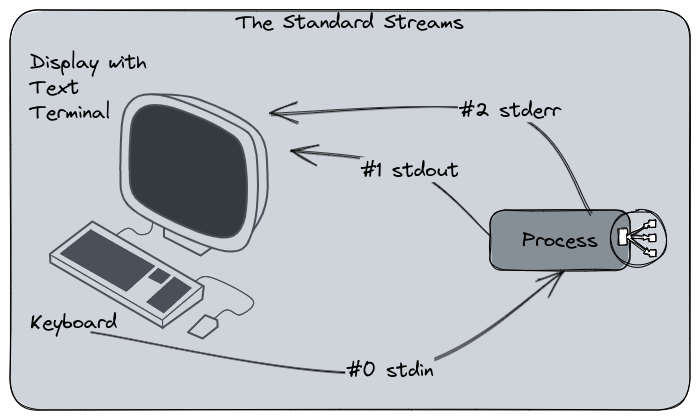
\includegraphics[width=10cm]{image/standard-stream-computer}
    \end{frame}

    \begin{frame}{Commandes de base}{Les flux standards dans le Shell Linux\cref{standard-stream}}
        \centering
        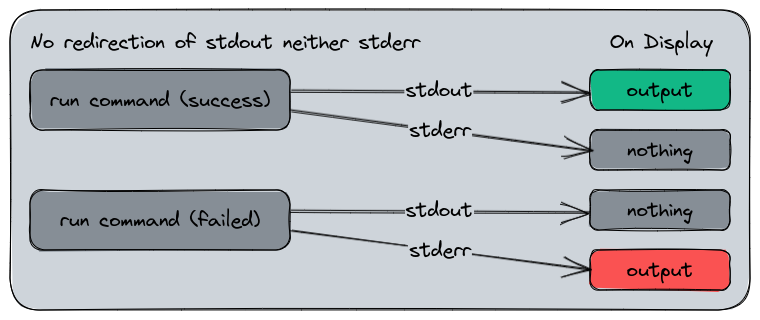
\includegraphics[width=10cm]{image/shell-stream-no-redirect}
    \end{frame}

    \begin{frame}{Commandes de base}{Opérateurs de redirection et piping\footnote{Five ways to use redirect operators in Bash, \url{https://www.redhat.com/sysadmin/redirect-operators-bash}}}
        \begin{footnotesize}
            \begin{itemize}
                \item \lstinline{>}~: Redirige la sortie standard vers un fichier.
                \item \lstinline{>>}~: Redirige la sortie standard vers un fichier en ajoutant le contenu à la fin.
                \item \lstinline{<}~: Redirige un fichier vers l'entrée standard.
                \item \lstinline{2>}~: Redirige la sortie d'erreur vers un fichier.
                \item \lstinline{&>}~: Redirige la sortie standard et d'erreur vers un fichier.
                \item \lstinline{|}~: Piping, redirige la sortie standard d'une commande vers l'entrée standard d'une autre.
            \end{itemize}
            À quoi ces opérateurs peuvent-ils servir~?
            \begin{center}
                
\includegraphics[width=3cm]{image/question-mark-on-a-blank-background.png}
            \end{center}
        \end{footnotesize}
    \end{frame}

    \begin{frame}{Commandes de base}{Opérateurs logiques}
        \begin{itemize}
            \item \lstinline{||}~: Exécute la commande suivante si la précédente a échoué.
            \item \lstinline{\&\&}~: Exécute la commande suivante si la précédente a réussi.
        \end{itemize}
        Ils peuvent définir le comportement d'un script et être utilisés dans des conditions.
        \bigbreak
        Lancer un \lstinline{sudo apt upgrade} uniquement si \lstinline{sudo apt update} \textbf{a fonctionné}.
        \bigbreak
        Logger un message d'erreur si \lstinline{ls klazkjhfzklefjh} \textbf{n'a pas fonctionné}.
        \bigbreak
        \centering
        
\includegraphics[width=3cm]{image/student-in-front-of-desktop}
    \end{frame}

    \begin{frame}{Commandes de base}{Exercice \execcounterdispinc{}~:}
        Le but est de créer un fichier source d'un script Shell en y ajoutant ligne par ligne les commandes~:
        \begin{itemize}
            \item Initier la création d'un script Shell nommé \lstinline{discover.sh} dans votre \textquote{home} avec un commentaire descriptif.
            \item Afficher un message indiquant que le \textquote{current working directory} va s'afficher.
            \item Afficher ce current working directory.
            \item Afficher un message indiquant que les fichiers et répertoires du répertoire courant vont s'afficher.
            \item Afficher la liste des fichiers et répertoires du répertoire courant.
        \end{itemize}

        Inutile donc indispensable~:
        \begin{itemize}
            \item Changer de répertoire pour aller dans le répertoire courant avec le pipe.
        \end{itemize}
    \end{frame}

    \begin{frame}{Commandes de base}{Exercice \execcounterdispinc{}~:}
        \begin{itemize}
            \item Rediriger la sortie standard de la commande \lstinline{ls} dans un fichier \lstinline{ls-output.txt}.
            \item Rediriger la sortie d'erreur de la commande \lstinline{ls} dans un fichier \lstinline{ls-error.txt}.
            \item Rediriger les deux flux dans un fichier \lstinline{ls-output-error.txt}.
            \item Rediriger le contenu du fichier \lstinline{ls-output.txt} dans l'entrée standard de la commande \lstinline{grep} pour filter sur un type d'extension de fichier.
        \end{itemize}
    \end{frame}

    \subsection{Commandes de traitement de données}\label{subsec:commandes-donnees}

    \begin{frame}{Commandes de traitement de données}{Les grands classiques}
        \begin{itemize}
            \item \lstinline{grep}~: Recherche de chaînes de caractères dans un fichier à l'aide d'une RegExp, une \textquote{Regular Expression}.
            Le nom vient de \textit{Global Regular Expression Print}.
            \item \lstinline{sed}~: Stream EDitor, éditeur de flux, permet de modifier le contenu d'un fichier.
            Le plus souvent à l'aide d'une RegExp également.
            Il peut substituer un pattern, supprimer une ligne, ajouter une ligne, \textit{etc}.
            \item \lstinline{awk}~: Traitement de texte, permet de lire un fichier ligne par ligne et de le traiter.
            Il est plus complexe, il a son propre langage de programmation.
            \item \lstinline{cut}~: Permet de découper un fichier en colonnes et de les sélectionner.
            \item \lstinline{sort}~: Trie les lignes d'un fichier.
            \item \lstinline{join}~: Joint les lignes de deux fichiers sur un champ commun.
            \item \lstinline{uniq}~: Supprime les lignes en double.
        \end{itemize}
    \end{frame}

    \subsubsection{Piping}\label{subsubsec:piping}
    \begin{frame}{Commandes de traitement de données}{L'histoire du piping}
        Les opérateurs de redirection et le piping fonctionnent toujours évidement avec ces commandes.
        \bigbreak
        \begin{columns}
            \centering
            \column{0.2\textwidth}
            
\includegraphics[width=2cm]{image/seat-and-watch}
            \column{0.8\textwidth}
            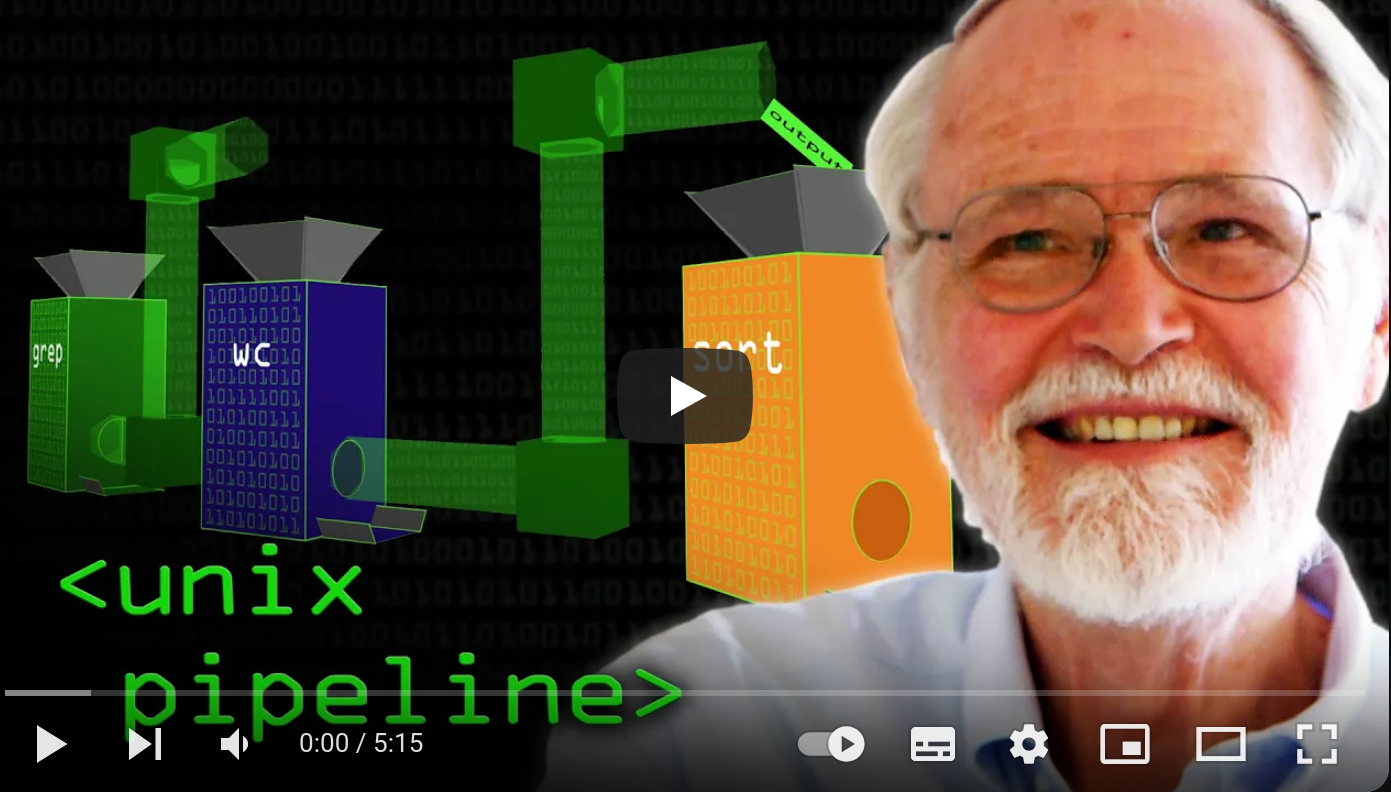
\includegraphics[width=9cm]{image/kernighan-piping-video} \\ \url{https://www.youtube.com/watch?v=bKzonnwoR2I} \\
        \end{columns}
    \end{frame}

    \subsubsection{grep}\label{subsubsec:grep}
    \begin{frame}[fragile]{Commandes de traitement de données}{\lstinline{grep}}
        Par exemple chercher une adresse mail dans un fichier.
        \bigbreak
        On valide d'abord la RegExp en ligne avec un utilitaire comme \url{https://regex101.com/}.
        \bigbreak
        Par exemple, pour chercher les connexions depuis une IP dans le fichier de ProFTP (un serveur FTP)~:
        \begin{lstlisting}[language=bash,basicstyle=\tiny\ttfamily]
$ grep -P 'from\s([0-9]{1,3}.[0-9]{1,3}.[0-9]{1,3}.[0-9]{1,3})' proftpd.log.1
2023-03-05 11:35:16,736 vps19562 proftpd[663168] vps19562.dreamhostps.com (104.156.155.30[104.156.155.30]): USER anonymous: no such user found from 104.156.155.30 [104.156.155.30] to~::ffff:66.33.201.239:21
2023-03-05 13:44:22,711 vps19562 proftpd[664214] vps19562.dreamhostps.com (183.127.77.34.bc.googleusercontent.com[34.77.127.183]): USER anonymous: no such user found from 183.127.77.34.bc.googleusercontent.com [34.77.127.183] to~::ffff:66.33.201.239:21
2023-03-05 21:18:51,926 vps19562 proftpd[669957] vps19562.dreamhostps.com (182.176.228.148[182.176.228.148]): USER local: no such user found from 182.176.228.148 [182.176.228.148] to~::ffff:66.33.201.239:21
2023-03-05 21:59:46,174 vps19562 proftpd[670340] vps19562.dreamhostps.com (107.150.102.211[107.150.102.211]): USER anonymous: no such user found from 107.150.102.211 [107.150.102.211] to~::ffff:66.33.201.239:21
2023-03-06 13:36:11,788 vps19562 proftpd[681605] vps19562.dreamhostps.com (116.62.233.35.bc.googleusercontent.com[35.233.62.116]): USER anonymous: no such user found from 116.62.233.35.bc.googleusercontent.com [35.233.62.116] to~::ffff:66.33.201.239:21
2023-03-07 10:19:49,666 vps19562 proftpd[695638] vps19562.dreamhostps.com (116.62.233.35.bc.googleusercontent.com[35.233.62.116]): USER anonymous: no such user found from 116.62.233.35.bc.googleusercontent.com [35.233.62.116] to~::ffff:66.33.201.239:21
        \end{lstlisting}
    \end{frame}

    \begin{frame}[fragile]{Commandes de traitement de données}{\lstinline{grep} pour le \textquote{Pattern Matching}}
        En rajouter l'option \lstinline{-o} pour avoir uniquement le pattern qui match~:
        \begin{lstlisting}[language=bash]
$ grep -oP 'from\s(\d{1,3}.\d{1,3}.\d{1,3}.\d{1,3})' proftpd.log.1
from 104.156.155.30
from 183.127.77.34
from 182.176.228.148
from 107.150.102.211
from 116.62.233.35
from 116.62.233.35
        \end{lstlisting}
        Uniquement sur les 10 premières lignes grâce à \lstinline{head}~:
        \begin{lstlisting}[language=bash]
$ grep -oP 'from\s(\d{1,3}.\d{1,3}.\d{1,3}.\d{1,3})' <(head -n 10 proftpd.log.1)
from 104.156.155.30
from 183.127.77.34
from 182.176.228.148
from 107.150.102.211
        \end{lstlisting}
        Expliquer cette dernière commande.
    \end{frame}

    \subsubsection{sed}\label{subsubsec:sed}
    \begin{frame}[fragile]{Commandes de traitement de données}{\lstinline{sed} la substitution}
        \lstinline{sed} a son propre langage de programmation avec \lstinline{s/} entre autre\footnote{\label{sed}Sed - An Introduction and Tutorial by Bruce Barnett, \url{https://www.grymoire.com/Unix/Sed.html}}.
        \bigbreak
        On peut anonymiser le fichier en remplaçant une chaine de caractère par une autre.
        \begin{lstlisting}[language=bash,basicstyle=\tiny\ttfamily]
$ head -n 3 proftpd.log.1
2023-03-05 00:17:11,880 vps19562 proftpX[653589] vps19562.dreamhostps.com: ProFTPD 1.3.6c (maint) (built Thu Feb 27 2020 19:34:56 UTC) standalone mode STARTUP
2023-03-05 00:47:51,132 vps19562 proftpX[653845] vps19562.dreamhostps.com (aurora.probe.onyphe.net[142.4.218.114]): USER anonymous: no such user found from aurora.probe.onyphe.net [142.4.218.114] to~::ffff:66.33.201.239:21
2023-03-05 00:55:14,666 vps19562 proftpX[655268] vps19562.dreamhostps.com (hodson.probe.onyphe.net[178.32.197.87]): USER anonymous: no such user found from hodson.probe.onyphe.net [178.32.197.87] to~::ffff:66.33.201.239:21
$ head -n 3 proftpd.log.1 | sed s/vps19562.dreamhostps.com/XXX/
2023-03-05 00:17:11,880 vps19562 proftpX[653589] XXX: ProFTPD 1.3.6c (maint) (built Thu Feb 27 2020 19:34:56 UTC) standalone mode STARTUP
2023-03-05 00:47:51,132 vps19562 proftpX[653845] XXX (aurora.probe.onyphe.net[142.4.218.114]): USER anonymous: no such user found from aurora.probe.onyphe.net [142.4.218.114] to~::ffff:66.33.201.239:21
2023-03-05 00:55:14,666 vps19562 proftpX[655268] XXX (hodson.probe.onyphe.net[178.32.197.87]): USER anonymous: no such user found from hodson.probe.onyphe.net [178.32.197.87] to~::ffff:66.33.201.239:21
        \end{lstlisting}
    \end{frame}

    \begin{frame}[fragile]{Commandes de traitement de données}{\lstinline{sed} la substitution avec \lstinline{s/}\cref{sed}}
        Pour anonymiser le fichier en remplaçant une chaine de caractère par une autre.
        On peut utiliser \lstinline{sed} pour substituer un pattern, donc une RegExp, avec l'option \lstinline{-E}, par une chaîne de caractère et donc anonymiser le fichier en remplaçant les IPv4 par \textquote{xxx.xxx.xxx.xxx}~:
        \begin{lstlisting}[language=bash,basicstyle=\tiny\ttfamily]
$ head -n 3 proftpd.log.1 | sed -E 's/\[[0-9]{1,3}.[0-9]{1,3}.[0-9]{1,3}.[0-9]{1,3}\]/[xxx.xxx.xxx.xxx]/g'
2023-03-05 00:17:11,880 vps19562 proftpX[653589] vps19562.dreamhostps.com: ProFTPD 1.3.6c (maint) (built Thu Feb 27 2020 19:34:56 UTC) standalone mode STARTUP
2023-03-05 00:47:51,132 vps19562 proftpX[653845] vps19562.dreamhostps.com (aurora.probe.onyphe.net[xxx.xxx.xxx.xxx]): USER anonymous: no such user found from aurora.probe.onyphe.net [xxx.xxx.xxx.xxx] to~::ffff:66.33.201.239:21
2023-03-05 00:55:14,666 vps19562 proftpX[655268] vps19562.dreamhostps.com (hodson.probe.onyphe.net[xxx.xxx.xxx.xxx]): USER anonymous: no such user found from hodson.probe.onyphe.net [xxx.xxx.xxx.xxx] to~::ffff:66.33.201.239:21
        \end{lstlisting}
    \end{frame}

    \begin{frame}[fragile]{Commandes de traitement de données}{\lstinline{sed} la supression avec \lstinline{/d}\cref{sed}}
        De la même manière et avec les mêmes options on peut supprimer une ligne qui match une chaine de caractère ou une RegExp~:
        \begin{lstlisting}[language=bash,basicstyle=\tiny\ttfamily]
$ head -n 3 proftpd.log.1
2023-03-05 00:17:11,880 vps19562 proftpX[653589] vps19562.dreamhostps.com: ProFTPD 1.3.6c (maint) (built Thu Feb 27 2020 19:34:56 UTC) standalone mode STARTUP
2023-03-05 00:47:51,132 vps19562 proftpX[653845] vps19562.dreamhostps.com (aurora.probe.onyphe.net[142.4.218.114]): USER anonymous: no such user found from aurora.probe.onyphe.net [142.4.218.114] to~::ffff:66.33.201.239:21
2023-03-05 00:55:14,666 vps19562 proftpX[655268] vps19562.dreamhostps.com (hodson.probe.onyphe.net[178.32.197.87]): USER anonymous: no such user found from hodson.probe.onyphe.net [178.32.197.87] to~::ffff:66.33.201.239:21
$ head -n 3 proftpd.log.1 | sed -E '/\[[0-9]{1,3}.[0-9]{1,3}.[0-9]{1,3}.[0-9]{1,3}\]/d'
2023-03-05 00:17:11,880 vps19562 proftpX[653589] vps19562.dreamhostps.com: ProFTPD 1.3.6c (maint) (built Thu Feb 27 2020 19:34:56 UTC) standalone mode STARTUP
$ head -n 3 proftpd.log.1 | sed '/vps19562.dreamhostps.com/d'
        \end{lstlisting}
        Il peut aussi supprimer une ligne spécifique, par exemple ici la première~:
        \begin{lstlisting}[language=bash,basicstyle=\tiny\ttfamily]
$ head -n 3 proftpd.log.1 | sed '1d'
2023-03-05 00:47:51,132 vps19562 proftpX[653845] vps19562.dreamhostps.com (aurora.probe.onyphe.net[142.4.218.114]): USER anonymous: no such user found from aurora.probe.onyphe.net [142.4.218.114] to~::ffff:66.33.201.239:21
2023-03-05 00:55:14,666 vps19562 proftpX[655268] vps19562.dreamhostps.com (hodson.probe.onyphe.net[178.32.197.87]): USER anonymous: no such user found from hodson.probe.onyphe.net [178.32.197.87] to~::ffff:66.33.201.239:21
        \end{lstlisting}
    \end{frame}

    \begin{frame}[fragile]{Commandes de traitement de données}{\lstinline{sed} plusieurs traitements}
        Plusieurs traitements peuvent être enchainés en les séparant par \lstinline{;}.
        Comme ici avec la suppression de la première ligne et l'anonymisation du serveur ensuite~:
        \begin{lstlisting}[language=bash,basicstyle=\tiny\ttfamily]
$ head -n 3 proftpd.log.1
2023-03-05 00:17:11,880 vps19562 proftpX[653589] vps19562.dreamhostps.com: ProFTPD 1.3.6c (maint) (built Thu Feb 27 2020 19:34:56 UTC) standalone mode STARTUP
2023-03-05 00:47:51,132 vps19562 proftpX[653845] vps19562.dreamhostps.com (aurora.probe.onyphe.net[142.4.218.114]): USER anonymous: no such user found from aurora.probe.onyphe.net [142.4.218.114] to~::ffff:66.33.201.239:21
2023-03-05 00:55:14,666 vps19562 proftpX[655268] vps19562.dreamhostps.com (hodson.probe.onyphe.net[178.32.197.87]): USER anonymous: no such user found from hodson.probe.onyphe.net [178.32.197.87] to~::ffff:66.33.201.239:21
$ head -n 3 proftpd.log.1 | sed -E '1d;s/\] .*.com/] XXX/g'
2023-03-05 00:47:51,132 vps19562 proftpX[653845] XXX (aurora.probe.onyphe.net[142.4.218.114]): USER anonymous: no such user found from aurora.probe.onyphe.net [142.4.218.114] to~::ffff:66.33.201.239:21
2023-03-05 00:55:14,666 vps19562 proftpX[655268] XXX (hodson.probe.onyphe.net[178.32.197.87]): USER anonymous: no such user found from hodson.probe.onyphe.net [178.32.197.87] to~::ffff:66.33.201.239:21
        \end{lstlisting}
    \end{frame}

    \subsubsection{cut}\label{subsubsec:cut}
    \begin{frame}[fragile]{Commandes de traitement de données}{\lstinline{cut} pour gérer les colonnes}
        Il est très utile pour travailler avec les fichiers de données comme CSV, TSV~.

        Il les découpe en colonnes et permet de sélectionner les colonnes voulues sur la base d'un séparateur spécifié avec l'option \lstinline{-d} ou \lstinline{--delimiter}.
        \bigbreak
        \lstinline{-f 1,3} pour sélectionner les colonnes 1 et 3~:
        \begin{lstlisting}[language=bash,basicstyle=\tiny\ttfamily]
$ head -n 3 employee.csv
"id";"name";"age";"salary";"dept_id"
0;"John";30;1000;0
1;"Jane";25;1500;0
$ cut employee.csv -f 1,3 --delimiter=';' | head -n 3
"id";"age"
0;30
1;25
        \end{lstlisting}
        \lstinline{-f 1-3} pour sélectionner les colonnes de 1 à 3~:
        \begin{lstlisting}[language=bash,basicstyle=\tiny\ttfamily]
$ cut employee.csv -f 1-3 --delimiter=';' | head -n 3
"id";"name";"age"
0;"John";30
1;"Jane";25
        \end{lstlisting}
    \end{frame}

    \subsubsection{sort}\label{subsubsec:sort}
    \begin{frame}[fragile]{Commandes de traitement de données}{\lstinline{sort} pour trier les lignes}
        \lstinline{sort} trie les lignes d'un fichier en se basant sur le premier champ par défaut ou en spécifiant un champ avec l'option \lstinline{-k} ou \lstinline{--key}.
        \begin{lstlisting}[language=bash,basicstyle=\tiny\ttfamily]
$ head employee.csv -n 4
"id";"name";"age";"salary";"dept_id"
0;"John";30;1000;0
1;"Jane";25;1500;0
2;"Doe";35;2000;1
        \end{lstlisting}
        Pour trier sur le salaire, la colonne 4, séparée par \textquote{;}~:
        \begin{lstlisting}[language=bash,basicstyle=\tiny\ttfamily]
$ sed 1d employee.csv | sort -k 4 --field-separator=';' | head -n 4
0;"John";30;1000;0
1;"Jane";25;1500;0
3;"Steeve";40;2000;0
2;"Doe";35;2000;1
        \end{lstlisting}
        Pour trier sur le salaire puis sur le nom en colonne 2~:
        \begin{lstlisting}[language=bash,basicstyle=\tiny\ttfamily]
$ sed 1d employee.csv | sort -k 4,2 --field-separator=';' | head -n 4
0;"John";30;1000;0
1;"Jane";25;1500;0
2;"Doe";35;2000;1
3;"Steeve";40;2000;0
        \end{lstlisting}
    \end{frame}

    \subsubsection{join}\label{subsubsec:join}
    \begin{frame}[fragile]{Commandes de traitement de données}{\lstinline{join} pour joindre 2 fichiers sur une clé}
        Jointure des fichiers CSV \lstinline{employee.csv} et \lstinline{dept.csv} sur la colonne \lstinline{dept_id} qui est commune aux 2~:
        \begin{lstlisting}[language=bash,basicstyle=\tiny\ttfamily]
$ join -1 1 -2 1 -t ';' -a 2 <(sed 1d employee.csv | sort -k 1 --field-separator=';') <(sed 1d dept.csv | sort -k 1 --field-separator=';')
0;"John";30;1000;0;"HR"
1;"Jane";25;1500;0;"Engineering"
2;"Doe";35;2000;1;"Finance"
$ join -1 1 -2 1 -t ';' -a 1 <(sed 1d employee.csv | sort -k 1 --field-separator=';') <(sed 1d dept.csv | sort -k 1 --field-separator=';')
0;"John";30;1000;0;"HR"
1;"Jane";25;1500;0;"Engineering"
2;"Doe";35;2000;1;"Finance"
3;"Steeve";40;2000;0
4;"Smith";40;2500;1
5;"Brown";45;3000;2
        \end{lstlisting}
        \begin{dangercolorbox}
            Les 2 doivent avoir exactement le même nombre de ligne~!
            Les 3 dernières lignes ont une correspondance dans le fichier \lstinline{dept.csv} mais aucune association n'est faite, car le fichier \lstinline{dept.csv} n'a que 3 lignes.

            Les clés d'associations doivent être triées, il y a donc toujours une étape avec \lstinline{sort} auparavant.
        \end{dangercolorbox}
    \end{frame}

    \begin{frame}{Commandes de traitement de données}{\lstinline{awk}}
        L'histoire et le bien fondé de \lstinline{awk} (12 premières minutes).
        \bigbreak
        \begin{columns}
            \centering
            \column{0.2\textwidth}
            
\includegraphics[width=2cm]{image/seat-and-watch}
            \column{0.8\textwidth}
            
\includegraphics[width=9cm]{image/coffee-with-bk} \\ \url{https://www.youtube.com/watch?v=GNyQxXw_oMQ} \\
        \end{columns}
    \end{frame}

    \begin{frame}{Commandes de traitement de données}{\lstinline{awk}}
        \begin{itemize}
            \item \textquote{The right tool for a job}.
            \item N'est même pas packagé, il vient dans toutes les distributions.
            \item Data orientated.
            \item Search a matching pattern.
            \item Add numbers.
            \item One liner.
            \item Fonctionne avec des \textquote{associative arrays}, donc similaire à des maps, dictionnaires\ldots.
        \end{itemize}
    \end{frame}

    \begin{frame}{Commandes de traitement de données}{Les traitement du type Unix, l'ETL du pauvre \emoji{rolling-on-the-floor-laughing}~?}
        Le data wrangling avant de remplir les bases des applicatifs~:
        \begin{center}
            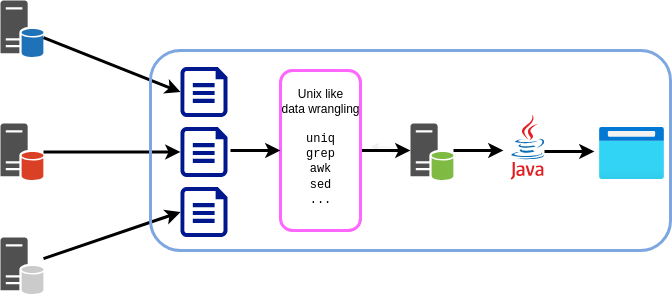
\includegraphics[width=11cm]{image/pre-traitement-unix.drawio}
        \end{center}
        Un ETL peut le faire mais beaucoup utilisent encore ces outils\ldots
    \end{frame}

    \begin{frame}{Commandes de traitement de données}{\lstinline{awk}, exercice \execcounterdispinc{}~:}
        Mais c'est aussi pour ajouter des nombres son créateur à dit, on peut donc faire de l'analytique avec~!
        \bigbreak
        Quelle est la somme des salaires par département dans le fichier \lstinline{employee.csv}~?
        \bigbreak
        \centering
        
\includegraphics[width=3cm]{image/question-mark-on-a-blank-background.png}
    \end{frame}

    \subsubsection{Exercice}\label{subsubsec:data-exercice}
    \begin{frame}{Commandes de traitement de données}{Exercice \execcounterdispinc{}~:}
        \begin{footnotesize}
            Cet exercice a pour objectif d'illustrer qu'un prétraitement avec ces commandes est efficace.
            Plus qu'un équivalent SQL~.
            \bigbreak
            Il est courant de limiter les données en base SQL aux besoins des programmes haut-niveau, d'un backend Java, CoBOL, PHP par exemple, pour ne pas surcharger les serveurs SQL~.
            \bigbreak
            Ces commandes ne remplacent pas SQL, car elles s'interfacent difficilement avec ces programmes haut-niveau.
            \bigbreak
            Par contre, elles peuvent traiter des flux de données avant de les mettre en base.
            L'exercice consiste à développer avec ces commandes l'équivalent des \href{https://github.com/DigicompClassesByPapIT/linux2/blob/main/sqlite-hr.sh}{traitements SQL de ce fichier}.
            Avec les données des fichiers \href{https://github.com/DigicompClassesByPapIT/linux2/blob/main/employee.csv}{\lstinline{employee.csv}} et \href{https://github.com/DigicompClassesByPapIT/linux2/blob/main/dept.csv}{\lstinline{dept.csv}}.

            Analyser~:
            \begin{itemize}
                \item Ce qui peut être qualifié d'\textquote{efficace}.
                \item Ce que cette \textquote{efficacité} apporte à l'entreprise.
                \item Quelle version SQL ou Shell est la plus sensible aux bugs et pourquoi~?
            \end{itemize}
        \end{footnotesize}
    \end{frame}

    \begin{frame}{Commandes de traitement de données}{Solution}
        Plusieurs solutions possibles sont dans le script Shell \url{https://github.com/DigicompClassesByPapIT/linux2/blob/main/join-using-awk.sh}.
        \bigbreak
        Elles sont équivalentes au SQL qui est dans le script \url{https://github.com/DigicompClassesByPapIT/linux2/blob/main/sqlite-hr.sh}.
        \bigbreak
        \centering
        
\includegraphics[width=3cm]{image/clever-lightbulb}
    \end{frame}

    \begin{frame}{Commandes de traitement de données}{Exercice \execcounterdispinc{}~:}
        De la même manière, préparer les fichiers suivants \href{https://github.com/DigicompClassesByPapIT/linux2/blob/main/receveur.csv}{\lstinline{receveur.csv}} et \href{https://github.com/DigicompClassesByPapIT/linux2/blob/main/porteur.csv}{\lstinline{porteur.csv}} pour qu'ils soient \textit{loadés} en la base SQL par le script \href{https://github.com/DigicompClassesByPapIT/linux2/blob/main/sqlite-load-bank.sh}{\lstinline{sqlite-load-bank.sh}}.
        \bigbreak
        Ces fichiers sont des flux de cartes bancaires.
        Un fichier du porteur de carte l'autre du commerçant aussi appelé receveur (de carte).
        \begin{itemize}
            \item Vérifier que toutes les transactions sont uniques, sinon arrêter le script en code retour 2.
            \item Il y a deux tables.
            Nettoyer les fichiers pour qu'ils soient le plus légers possibles lors de la manipulation.
            Faites deux branches, une pour chaque table et supprimer les colonnes inutiles.
            \item Vérifier que les fichiers sont bien nettoyés.
            \item Sommer les montants dans un fichier, par identifiant de banque dans un fichier et par identifiant de client dans un autre.
            \item Loader les fichiers dans la base.
        \end{itemize}
    \end{frame}

    \subsubsection{Equivalence SQL - Shell}\label{subsubsec:equi-sql-shell}
    \begin{frame}{Commandes de traitement de données}{Equivalence SQL - Shell}
        De nombreux traitements de données ne nécessitent pas toujours de SQL, ils ont leur équivalent en Shell~:
        \begin{table}[ht]
            \centering
            \begin{tabular}{|c|c|}
                \hline
                \textbf{SQL}         & \textbf{Shell}                    \\
                \hline
                \lstinline{SELECT}   & \lstinline{cut}                   \\
                \hline
                \lstinline{DELETE}   & \lstinline{sed}                   \\
                \hline
                \lstinline{UPDATE}   & \lstinline{sed}, \lstinline{awk}  \\
                \hline
                \lstinline{INSERT}   & \lstinline{<}                     \\
                \hline
                \lstinline{WHERE}    & \lstinline{grep}                  \\
                \hline
                \lstinline{JOIN}     & \lstinline{join}, \lstinline{awk} \\
                \hline
                \lstinline{GROUP BY} & \lstinline{awk}                   \\
                \hline
                \lstinline{ORDER BY} & \lstinline{sort}                  \\
                \hline
            \end{tabular}
%\caption{SQL functions and their Shell commands equivalents}
        \end{table}
        Dans une grande banque d'investissement française, chaque soir, le data center d'IBM facture des dizaines de milliers d'EUR pour les batchs qui traitent les données du jour\ldots
    \end{frame}

    \subsubsection{Les variantes}\label{subsubsec:variantes}

    \begin{frame}{Commandes de traitement de données}{Variantes de ces outils}
        Ces outils sont open-source et ont d'innombrables variantes~:
        \begin{itemize}
            \item \lstinline{egrep}~: Extended \lstinline{grep}.
            \item \lstinline{gsed}~: La version sous licence GNU de \lstinline{sed}.
            \item \lstinline{gawk}~: La version sous licence GNU de \lstinline{awk}.
            \item \lstinline{bawk}~: Binary \lstinline{awk}, pour parser des fichiers binaires.
            \item \lstinline{busybox}~: Ils ont tous une version dans cette boîte à outils.
        \end{itemize}
        \bigbreak
        Quel est l'intérêt de traiter des fichiers binaires~?
        \bigbreak
        \centering
        
\includegraphics[width=3cm]{image/question-mark-on-a-blank-background.png}
    \end{frame}

    \begin{frame}[fragile]{Commandes de traitement de données}{Variantes de ces outils}
        Dans les exemples précédents, nous n'avons manipulé que des données issues de fichier texte.
        Les données numériques prennent moins de place en binaire.
        \begin{lstlisting}[language=python]
from sys import getsizeof
from struct import pack
print("lentgh of the string:", getsizeof("65535")) # lentgh of the string: 46
print("lentgh of the struct:", getsizeof(pack(">H", 0xffff))) # lentgh of the struct: 35
        \end{lstlisting}
        La valeur d'un octet est comprise entre 0 et 255, mais pour obtenir du texte, on passe par une table de correspondance, un encodage, qui donnera un seul caractère.
        La valeur numérique la plus élevée pour ce même octet en texte est donc 9.
        \bigbreak
        Pour des soucis de performance, de coût (du cloud), il n'est pas rare que les formats de données soit binaires.
    \end{frame}

    \subsection{Synchronisation avec rsync}\label{subsec:rsync-syncro}

    \begin{frame}{Réseau}{rsync}
        \begin{columns}
            \column{0.7\textwidth}
            Rsync est un outil de synchronisation de fichiers qui permet de copier des fichiers locaux ou distants.
            Mais son réel atout est bien pour la synchronisation de fichiers, en local on a \lstinline{cp} pour copier ou pour pousser à travers le SSH sans juste synchroniser il existe \lstinline{scp}\ldots
            \bigbreak
            Il est souvent utilisé pour synchroniser des fichiers entre un serveur et un client SSH, donc de ne déplacer que le nécessaire.
            \bigbreak
            Par exemple les IDE JetBrains peuvent synchroniser le code avec d'autres machines pour le déploiement sur les environnements de développement/testing, \textit{etc}.
            \column{0.3\textwidth}
            \centering
            
\includegraphics[width=4cm]{image/hdd-synchronous}
        \end{columns}
    \end{frame}

    \begin{frame}[fragile]{Réseau}{La commande \lstinline{rsync}\footnote{Rsync Command in Linux with Examples, \url{https://linuxize.com/post/how-to-use-rsync-for-local-and-remote-data-transfer-and-synchronization/}}}
        La syntaxe générale de la commande est \lstinline{rsync <OPTION(S)> <SRC> <DEST>}.
        Pour synchroniser des fichiers locaux sur une autre machine (qui est donc serveur SSH) la destination est préfixée par le user et l'hôte~:
        \bigbreak
        \begin{lstlisting}[language=bash]
$ rsync -a /chemin/vers/mon-dossier/ utilisateur@serveur:/chemin/vers/mon-dossier/
        \end{lstlisting}
        Pour synchroniser des fichiers distants depuis une autre machine la source est préfixée par le user et l'hôte~:
        \begin{lstlisting}[language=bash]
$ rsync -a utilisateur@serveur:/chemin/vers/mon-dossier/ /chemin/vers/mon-dossier/
        \end{lstlisting}
        Pour spécifier le port SSH si différent de 22, il faut rajouter un morceau de commande SSH en argument \lstinline{-e "ssh -p <port>"}.
    \end{frame}

    \begin{frame}{Réseau}{Exercice \execcounterdispinc}
        Utiliser \lstinline{rsync} pour synchroniser un dossier entre deux VMs.
        \begin{itemize}
            \item Envoyer un fichier sur la VM de votre camarade.
            \item Vérifier que le fichier transféré est bien synchronisé donc identique avec \lstinline{sha256sum} ou \lstinline{md5sum}.
            \item Récupérer un fichier de la VM de votre camarade.
            \item Vérifier que le fichier transféré est bien synchronisé donc identique avec \lstinline{sha256sum} ou \lstinline{md5sum}.
            \item À l'image d'un backup périodique, utiliser crontab et \lstinline{rsync} pour synchroniser un fichier toutes les 5 minutes.
        \end{itemize}
        \begin{center}
            
\includegraphics[width=3cm]{image/student-in-front-of-desktop}
        \end{center}
    \end{frame}


    \section{Scripts Shell}\label{sec:scripting-shell}


    \begin{frame}{Scripts Shell}{Définition}
        Les scripts Shell sont des fichiers de texte avec l'extension \lstinline{.sh}, contenant des commandes Shell.
        Ils sont exécutés par un interpréteur de commandes Shell.
        \bigbreak
        Ils peuvent utiliser tous les commandes vues précédemment, toutes celles dans le \textquote{path}, tous les exécutables de la machine tant que le script a les droits adéquats.
        \bigbreak
        \begin{columns}
            \column{0.6\textwidth}
            Comme vue précédemment, il existe des variantes de Shell.
            Ce cours se focalise sur le Bash, un Shell populaire et plus complet que le Shell POSIX, idéal pour le scripting.
            \column{0.4\textwidth}
            \centering
            
\includegraphics[width=4cm]{image/bash-logo}
        \end{columns}
    \end{frame}

    \begin{frame}{Scripts Shell}{Usages}
        Ils sont fréquemment utilisés pour~:
        \begin{itemize}
            \item Des tâches répétitives, lancer un programme ou un script.
            \item Des tâches de maintenance, \lstinline{mysqlcheck}.
            \item Des tâches de backup, \lstinline{mysqldump}.
            \item Des tâches de déploiement, \lstinline{rsync} pour pousser du code.
            \item Des tâches de nettoyage, \lstinline{docker prune -a}.
            \item Des tâches de monitoring, récolté des données pour RRDTool.
            \item Des tâches de sécurité, extraire des données de logs et les envoyer pour analyse.
            \item \textit{Many more}.
        \end{itemize}
        Shellcheck\footnote{https://www.shellcheck.net/, \url{https://www.shellcheck.net/}} qui aide à vérifier la syntaxe et la qualité du code.
        Il a des extensions pour la plupart des IDE~.
    \end{frame}

    \begin{frame}{Scripts Shell}{Usages déconseillés}
        C'est un langage interprété et simple en comparaison des langages de programmation comme Python, Java, C++, \textit{etc}.

        Il faut trouver un autre environnement de développement pour~:
        \begin{itemize}
            \item Des architectures complexes qui nécessitent une modularité du code, car il n'y pas de système d'import perfectionné.
            Seulement \lstinline{source}
            \item Des performances critiques, car c'est un langage interprété.
            \item Des applications ayants des dépendances car aucun package manager.
            \item Des algorithmes complexes, car il n'éxiste aucun débuggeur sous Bash ou Shell!
            Il faut ajouter des outputs du type \lstinline{echo} ou \lstinline{printf} pour débugger ou des options.
        \end{itemize}
        \bigbreak
        Les scripts Shell doivent rester simples.
    \end{frame}

    \begin{frame}[fragile]{Scripts Shell}{Les performances}
        \url{https://notes-on-cython.readthedocs.io/en/latest/} nous explique l'importance de l'algorithme dans les performances.
        Un bon algorithme Python, donc interprété, est plus rapide qu'un mauvais algorithme C qui est compilé.
        \bigbreak
        Malheureusement, les performances Shell sont si mauvaise que même un bon algorithme Shell est plus lent qu'un mauvais algorithme Python.
        \begin{lstlisting}[language=bash]
$ time bash fibo_cached.sh 20
6765

real    0m7,030s
user    0m5,426s
sys     0m2,149s
$ time python3 fibo.py 20
6765

real    0m0,013s
user    0m0,007s
sys     0m0,006s
        \end{lstlisting}
    \end{frame}

    \begin{frame}{Scripts Shell}{Outil de choix pour les scripts simples}
        \begin{center}
            
\includegraphics[width=5cm]{image/pinguin-hugging-shell}
        \end{center}
        Ceci étant dit, sa syntaxe et son outillage simple en font un outils de scripting idéal pour tous.
        Par opposition à d'autres langages nécessitant une expertise plus poussée.
    \end{frame}


    \section{Syntaxe Shell}\label{sec:syntaxe-shell}

    \begin{frame}{Syntaxe Shell}{Variables et Paramètres\footnote{\label{devhint-bash}Bash scripting cheatsheet, \url{https://devhints.io/bash}}}
        \bigbreak
        \begin{itemize}
            \item Définir une variable~: \lstinline{NOM=valeur}
            \item Définir une constante~: \lstinline{readonly NOM=valeur}
            \item Référencer~: \lstinline{$NOM}
            \item Paramètres spéciaux~:
            \begin{itemize}
                \item \lstinline{$\#} - Nombre d'arguments
                \item \lstinline{$@} - Tous les arguments positionnels comme chaînes séparées
                \item \lstinline{$*} - Tous les arguments positionnels comme une seule chaîne
                \item \lstinline{$1}, \lstinline{$2}, \textit{etc} - Arguments positionnels
                \item \lstinline{$_} - Dernier argument du dernier processus
            \end{itemize}
        \end{itemize}
    \end{frame}

    \begin{frame}[fragile]{Syntaxe Shell}{Boucles\cref{devhint-bash}}
        \begin{itemize}
            \item Boucle for de base~:
            \begin{lstlisting}[language=bash]
for i in /etc/rc.*; do
    echo "$i"
done
            \end{lstlisting}
            \item Boucle de style C~:
            \begin{lstlisting}[language=bash]
for ((i = 0 ; i < 100 ; i++)); do
    echo "$i"
done
            \end{lstlisting}
            \item Boucle while~:
            \begin{lstlisting}[language=bash]
while read -r ligne; do
    echo "$ligne"
done < fichier.txt
            \end{lstlisting}
        \end{itemize}
    \end{frame}

    \begin{frame}{Syntaxe Shell}{Conditions\cref{devhint-bash}}
        \begin{itemize}
            \item Conditions sur les chaînes~:
            \begin{itemize}
                \item \lstinline{[[ -z CHAINE ]]} - Chaîne vide
                \item \lstinline{[[ CHAINE == CHAINE ]]} - Chaînes égales
            \end{itemize}
            \item Conditions numériques~:
            \begin{itemize}
                \item \lstinline{[[ NUM -lt NUM ]]} - Moins que
                \item \lstinline{(( NUM < NUM ))} - Comparaison numérique
            \end{itemize}
            \item Conditions sur les fichiers~:
            \begin{itemize}
                \item \lstinline{[[ -e FICHIER ]]} - Le fichier existe
                \item \lstinline{[[ -x FICHIER ]]} - Le fichier est exécutable
            \end{itemize}
            Opérateurs logiques~:
            \begin{itemize}
                \item \lstinline{[[ ! EXPR ]]} - Non
                \item \lstinline{[[ EXPR1 && EXPR2 ]]} - Et
                \item \lstinline{[[ EXPR1 || EXPR2 ]]} - Ou
            \end{itemize}
        \end{itemize}
    \end{frame}

    \begin{frame}[fragile]{Syntaxe Shell}{Tableaux et Dictionnaires\cref{devhint-bash}}
        \begin{itemize}
            \item Définir des tableaux~:
            \begin{lstlisting}[language=bash]
Fruits=('Pomme' 'Banane' 'Orange')
            \end{lstlisting}
            \item Accéder aux éléments~:
            \begin{lstlisting}[language=bash]
echo "${Fruits[0]}" # Pomme
            \end{lstlisting}
            \item Définir des dictionnaires ou \textit{associative array}~:
            \begin{lstlisting}[language=bash]
declare -A sons
sons[chien]="aboyer"
            \end{lstlisting}
            \item Accéder aux valeurs~:
            \begin{lstlisting}[language=bash]
echo "${sons[chien]}" # aboyer
aboyer
            \end{lstlisting}
        \end{itemize}
    \end{frame}

    \begin{frame}[fragile]{Syntaxe Shell}{Fonctions et Gestion des Erreurs\cref{devhint-bash}}
        \begin{itemize}
            \item Définir une fonction~:
            \begin{lstlisting}[language=bash,basicstyle=\ttfamily\tiny]
mafunc() {
    echo "Bonjour $1"
}
            \end{lstlisting}
            \lstinline{$1} est le premier argument passé à la fonction.
            \item Retourner des valeurs avec \lstinline{echo}~:
            \begin{lstlisting}[language=bash,basicstyle=\ttfamily\tiny]
$ echo $(mafunc "Jean")
Bonjour Jean
            \end{lstlisting}
            \item Gestion des erreurs~:
            \begin{lstlisting}[language=bash,basicstyle=\ttfamily\tiny]
mafunc() {
    return 1
}
if mafunc; then
    echo "Succès"
else
    echo "Échec"
fi
Échec
            \end{lstlisting}
            \lstinline{return} est utilisé pour retourner un code retour mais aucune autre valeur.
            Il est compris entre 0 et 255.
        \end{itemize}
    \end{frame}

    \begin{frame}[fragile]{Opérateurs arithmétiques}
        \begin{itemize}
            \item Addition~: \lstinline{a=$((1 + 2))}
            \item Soustraction~: \lstinline{a=$((1 - 2))}
            \item Multiplication~: \lstinline{a=$((1 * 2))}
            \item Division~: \lstinline{a=$((1 / 2))}
            \item Modulo~: \lstinline{a=$((1 % 2))}
            \item Incrémenter~: \lstinline{a=$((a + 1))} ou \lstinline{((a+=1))}
            \item Décrémenter~: \lstinline{a=$((a - 1))} ou \lstinline{((a-=1))}
        \end{itemize}
    \end{frame}

    \begin{frame}[fragile]{Divers\cref{devhint-bash}}
        \begin{itemize}
            \item Commentaires~:
            \begin{lstlisting}[language=bash]
# Ceci est un commentaire
            \end{lstlisting}
            \item Expansion d'historique~:
            \begin{lstlisting}[language=bash]
!!              # Répéter la dernière commande
!-<chiffre>     # Répéter la n-ième commande de l'historique
            \end{lstlisting}
        \end{itemize}
    \end{frame}


    \begin{frame}[fragile]{Les différentes parenthèses en Bash\footnote{\label{penthesisbash}Référence rapide des supports Bash, \url{https://dev-to.translate.goog/rpalo/bash-brackets-quick-reference-4eh6?_x_tr_sl=en&_x_tr_tl=fr&_x_tr_hl=fr&_x_tr_pto=rq}}}{Crochets simples \texttt{[ ]}}
        \begin{small}
            \begin{itemize}
                \item Utilisés pour des tests de conditions comme la commande \lstinline{test}.
                \item Supporte les tests sur les fichiers, les chaînes de caractères et les nombres.
                \item Exemple :
                \begin{lstlisting}[language=bash]
if [ -f fichier.txt ]; then
    echo "Le fichier existe."
else
    echo "Le fichier n'existe pas"
fi
Le fichier n'existe pas
                \end{lstlisting}
                \begin{dangercolorbox}
                    Supporte l'expansion de nom de fichier\footnotemark{} avec \lstinline{[ -f *.txt ];} donc peut causer des erreurs s'il y a plusieurs résultats.
                    En effet on aura une liste de fichiers et non un fichier, d'où une erreur de syntaxe Bash.
                \end{dangercolorbox}
            \end{itemize}
        \end{small}
        \footnotetext{Filename Expansion, \url{https://www.gnu.org/software/bash/manual/html_node/Filename-Expansion.html}}
    \end{frame}

    \begin{frame}[fragile]{Les différentes parenthèses en Bash\cref{penthesisbash}}{Doubles crochets \texttt{[[ ]]}}
        \begin{itemize}
            \item Plus puissant que les crochets simples.
            \item Supporte les expressions régulières et les comparaisons avancées.
            \item Ne subit pas l'expansion des fichiers comme les crochets simples.
            \item Exemple :
            \begin{lstlisting}[language=bash]
[[ $chaine =~ ^[a-z]+$ ]]
            \end{lstlisting}
        \end{itemize}
    \end{frame}

    \begin{frame}[fragile]{Les différentes parenthèses en Bash\cref{penthesisbash}}{Accolades simples \texttt{\{\}}}
        \begin{itemize}
            \item Utilisées pour l'expansion de chaînes ou la création de séquences.
            \item Permet de générer rapidement des listes.
            \item Exemple :
            \begin{lstlisting}[language=bash]
$ echo {1..5}  # Produit : 1 2 3 4 5
1 2 3 4 5
$ echo {a..e}  # Produit : a b c d e
a b c d e
            \end{lstlisting}
        \end{itemize}
    \end{frame}

    \begin{frame}[fragile]{Les différentes parenthèses en Bash\cref{penthesisbash}}{Dollar Accolades \texttt{\$\{\}}}
        \begin{itemize}
            \item Utilisées pour l'expansion de variables.
            \item Permet des manipulations avancées des variables (longueur, remplacement, sous-chaîne).
            \item Exemple de \textit{slicing}:
            \begin{lstlisting}[language=bash]
$ nom="Ryan"
$ echo ${nom:1:3}  # Entre 1 et 3
yan
$ echo ${nom:1} # À partir de 1 inclus
yan
$ echo ${nom::3} # Jusqu'à 3 exclu
Rya
            \end{lstlisting}
        \end{itemize}
    \end{frame}

    \begin{frame}[fragile]{Les différentes parenthèses en Bash\cref{penthesisbash}}{Doubles parenthèses \lstinline{(( ))}}
        \begin{itemize}
            \item Utilisées pour les évaluations arithmétiques.
            \item Permet d'effectuer des opérations mathématiques directement dans le script.
            \item Exemple :
            \begin{lstlisting}[language=bash]
$ resultat=$((3 + 5))
$ echo $resultat  # Produit : 8
8
            \end{lstlisting}
        \end{itemize}
    \end{frame}

    \begin{frame}[fragile]{Les différentes parenthèses en Bash\cref{penthesisbash}}{\lstinline{<<} Heredocs}
        \begin{itemize}
            \item Permet d'insérer du texte multi-ligne dans un script Bash.
            \item Utilisé pour les scripts ou les messages longs.
            \item Exemple :
            \begin{lstlisting}[language=bash]
$ cat <<EOF
Ceci est un texte
multi-ligne.
EOF
Ceci est un texte
multi-ligne.
            \end{lstlisting}
        \end{itemize}
    \end{frame}

    \begin{frame}[fragile]{Exercice\footnote{\label{fibo-ross}How Fast are \lstinline{def} \lstinline{cdef} \lstinline{cpdef}?, \url{https://notes-on-cython.readthedocs.io/en/latest/fibo_speed.html}} \execcounterdispinc{}}
        Sachant que la commande \lstinline{source} permet de charger un script Shell dans le Shell en cours d'utilisation.

        Écrire une fonction récursive qui calcul la série de Fibonacci simple à l'image du pseudo-code suivant~:
        \begin{footnotesize}
            \begin{verbatim}
function fib(n)
    if n < 2 then
        return n
    else
        val = fib(n-2) + fib(n-1)
        return val
    end if
end function
            \end{verbatim}
        \end{footnotesize}
        \begin{itemize}
            \item Quel(s) Shell peut-on utiliser~?
            \item Charger la function avec \lstinline{source} pour l'utiliser dans votre Shell.
        \end{itemize}
    \end{frame}

    \begin{frame}[fragile]{Une des solutions possibles en Shell Posix}
        \begin{lstlisting}[language=bash]
#!/bin/sh

fibo() {
    n=$1
    if [ "$n" -lt 2 ]; then
        echo "$n"
        return
    fi

    val1=$(fibo $((n - 1)))
    val2=$(fibo $((n - 2)))

    val=$((val1 + val2))

    echo "$val"
}

fibo "$1"
        \end{lstlisting}
    \end{frame}

    \begin{frame}[fragile]{Exercice\cref{fibo-ross} \execcounterdispinc{}}
        Écrire une fonction récursive qui calcul la série de Fibonacci avec caching à l'image du pseudo-code suivant~:
        \begin{footnotesize}
            \begin{verbatim}
function fib_cached(n, cache)
    if n < 2 then
        return n
    elese
        if cache contains n then
            return cache[n]
        else
            val = fib_cached(n-2, cache) + fib_cached(n-1, cache)
            cache[n] = val
            return val
        end if
    end if
end function
            \end{verbatim}
        \end{footnotesize}
        \begin{itemize}
            \item Quel(s) Shell peut-on utiliser~?
            \item Charger la function avec \lstinline{source} pour l'utiliser dans votre Shell.
        \end{itemize}
    \end{frame}

    \begin{frame}[fragile]{Une des solutions possibles en Bash}
        \begin{lstlisting}[language=bash]
#!/bin/bash
declare -A cache  # Declare an associative array for caching

fibo_cached() {
    local n=$1
    if (( n < 2 )); then
        echo "$n"
        return
    fi

    if [[ -n "${cache[$n]}" ]]; then
        echo "${cache[$n]}"
        return
    fi

    local val1=$(fibo_cached $((n - 1)))
    local val2=$(fibo_cached $((n - 2)))
    local val=$((val1 + val2))
    cache[$n]=$val  # Cache the result
    echo "$val"
}

fibo_cached "$1"
        \end{lstlisting}
    \end{frame}

    \begin{frame}[fragile]{Exercice\cref{fibo-ross} \execcounterdispinc{}}
        Comparer le temps execution de la fonction récursive simple et de la fonction récursive avec caching en utilisant la commande \lstinline{time}.

        La syntaxe de la commande \lstinline{time} est la suivante~:
        \begin{lstlisting}[language=bash]
$ time <commande>
        \end{lstlisting}
        \begin{itemize}
            \item Y-a-til une différence significative de performance~?
            \item Si oui, laquelle et pourquoi~?
        \end{itemize}
        \begin{center}
            
\includegraphics[width=3cm]{image/student-in-front-of-desktop}
        \end{center}
    \end{frame}

    \begin{frame}{Editeur Shell}{VS Code de Microsoft et ShellCheck}
        L'objectif de cette section est d'éditer un script Shell dans un environment dédié au développement.
        Un environment qui contient tous les outils nécessaires pour trouver rapidement les erreurs de syntaxe et tester son script.
        \bigbreak
        Pour le lancer taper \textquote{code} dans la barre de recherche de Linux ou \lstinline{code .} dans un terminal pour le lancer dans le répertoire courant.
        \begin{itemize}
            \item Ouvrir VS Code.
            \item Ouvrir ou créer le fichier contenant le code Shell.
            \item Trouver un plugin dédié au développement Shell dans la \textit{marketplace}.
            Ici \textquote{ShellCheck} pour la vérification de la syntaxe.
            En lisant la documentation on comprend que c'est une intégration de ShellCheck qui vient sans ce dernier sur certaines plateformes.
            Il faut installer ShellCheck.
            \item Installer le plugin.
            \item Tester le plugin en écrivant sciemment un code erroné.
        \end{itemize}
    \end{frame}

    \begin{frame}{Editeur Shell}{VS Code de Microsoft}
        \centering
        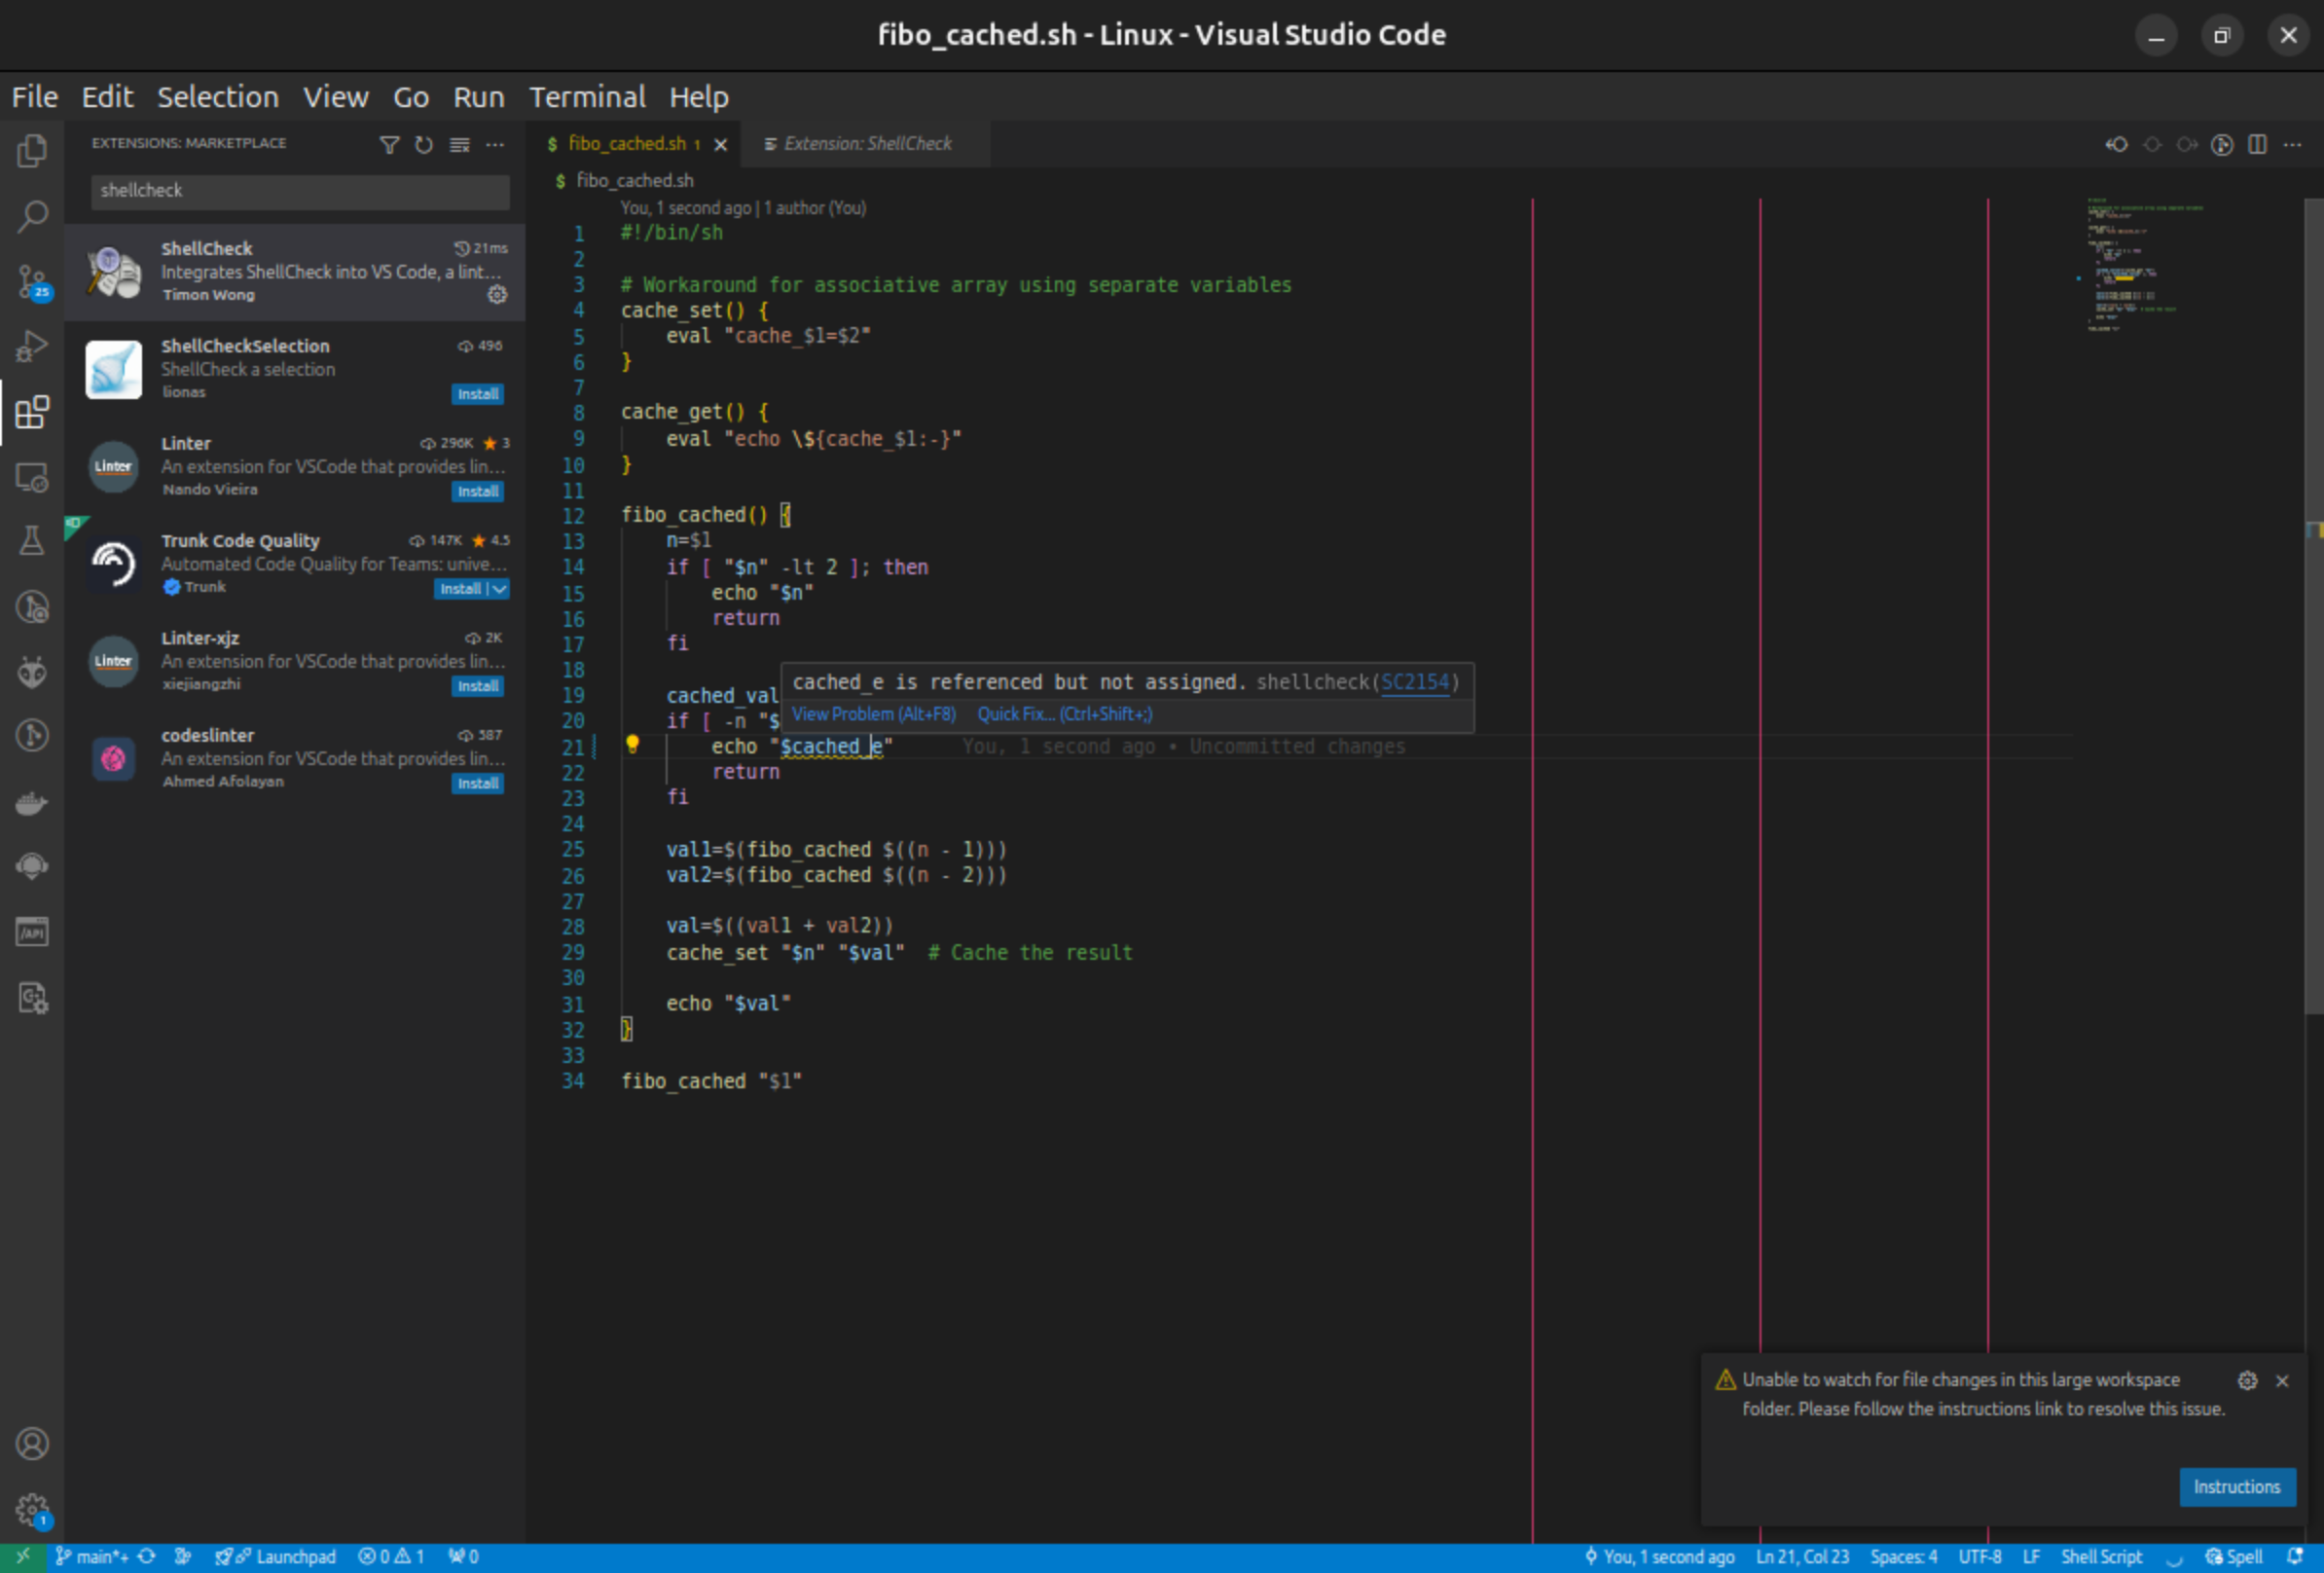
\includegraphics[width=11cm]{image/shellcheck-install}
    \end{frame}

    \begin{frame}[fragile]{Editeur Shell}{VS Code de Microsoft et ShellCheck}
        Les erreurs/warning qui sont en ligne apparaissent dans l'IDE VS Code.
        \begin{lstlisting}[language=bash,basicstyle=\tiny\ttfamily]
$ shellcheck fibo.ksh

In fibo.ksh line 7:
echo $n
^-- SC2086 (info): Double quote to prevent globbing and word splitting.

Did you mean:
echo "$n"


In fibo.ksh line 11:
typeset val1=$(fibo $((n - 1)))
^--^ SC2034 (warning): val1 appears unused. Verify use (or export if used externally).
^--^ SC2155 (warning): Declare and assign separately to avoid masking return values.


In fibo.ksh line 12:
typeset val2=$(fibo $((n - 2)))
^--^ SC2034 (warning): val2 appears unused. Verify use (or export if used externally).
^--^ SC2155 (warning): Declare and assign separately to avoid masking return values.


In fibo.ksh line 14:
typeset val=$((valeur1 + valeur2))
^-----^ SC2154 (warning): valeur1 is referenced but not assigned.
^-----^ SC2154 (warning): valeur2 is referenced but not assigned.
        \end{lstlisting}
    \end{frame}

    \begin{frame}{Editeur Shell}{VS Code de Microsoft et ShellCheck}
        \centering
        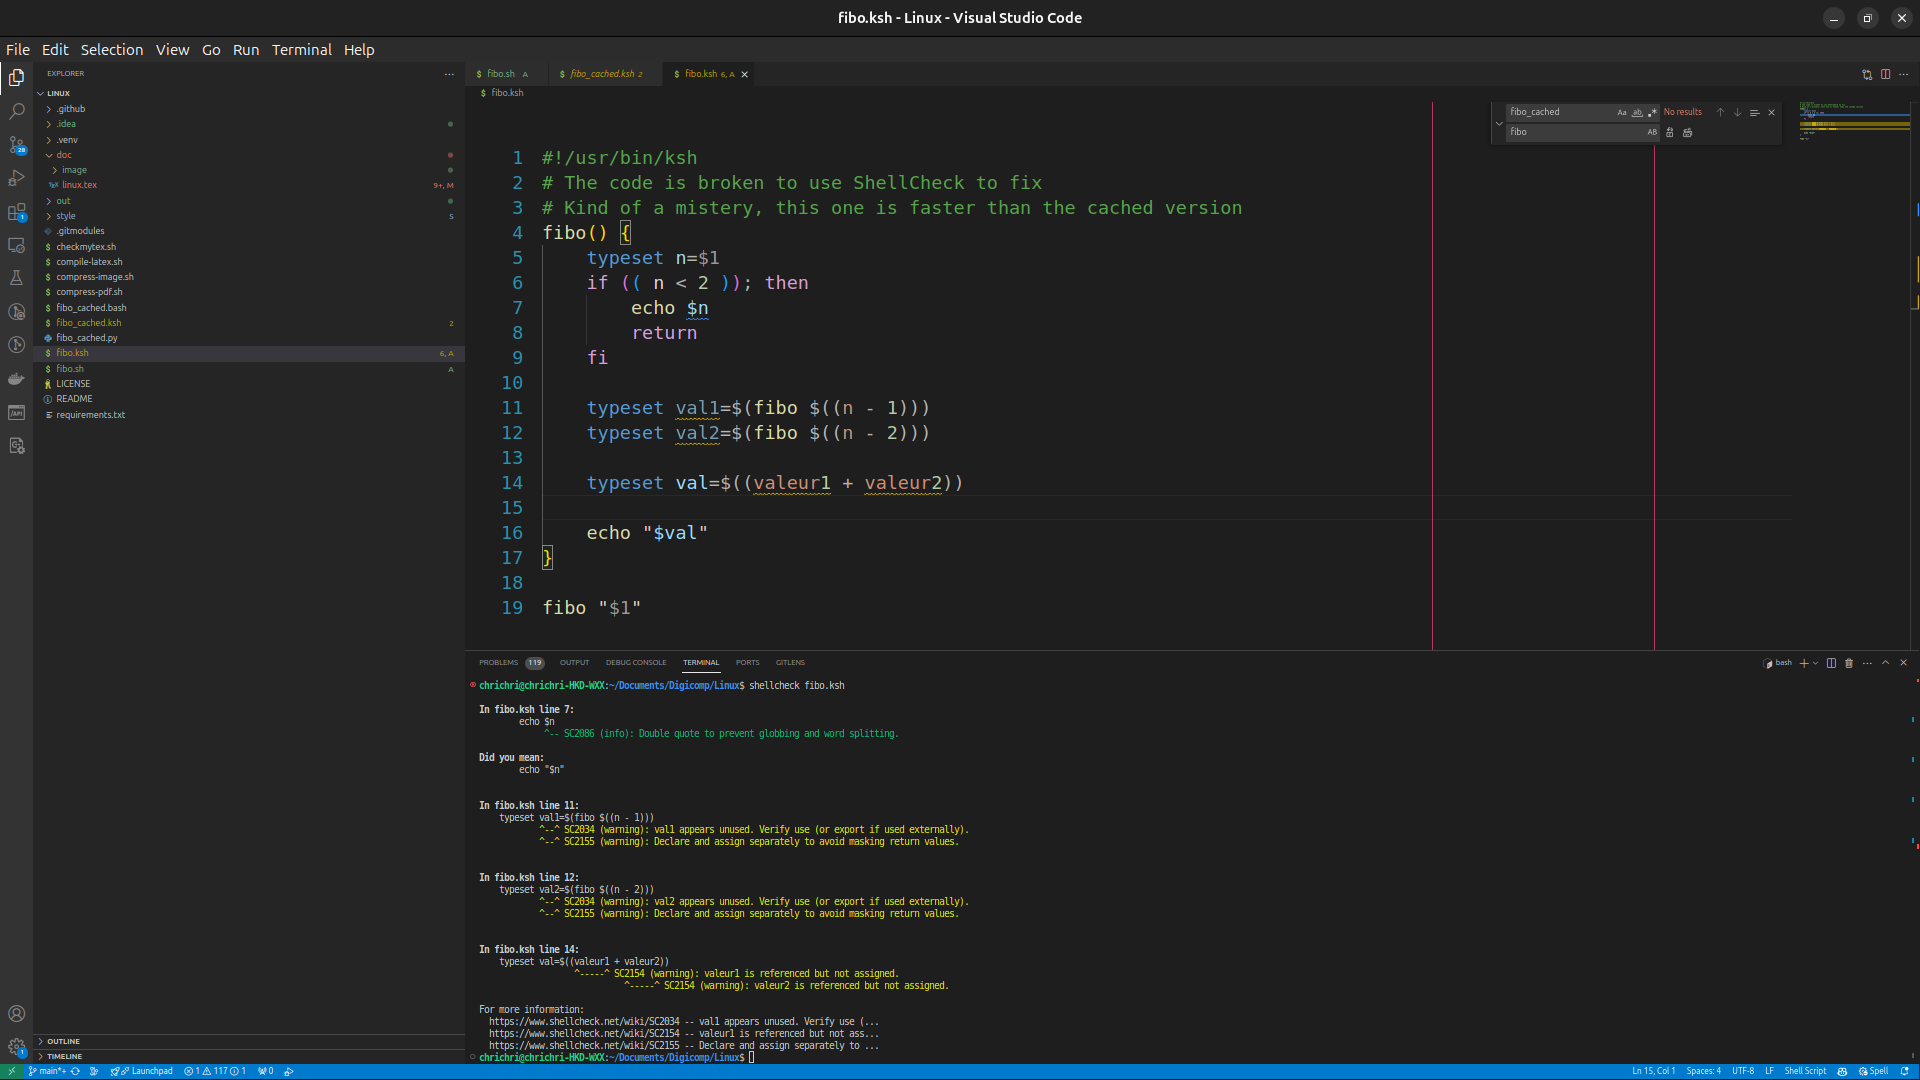
\includegraphics[width=12cm]{image/shellcheck-warning}
    \end{frame}

    \begin{frame}{Editeurs Shell}{Exercice \execcounterdispinc}
        Cette exercice a pour but d'illustrer que les éditeurs fournissent une aide pour tout type de langage.
        \begin{itemize}
            \item Installer VS Code.
            \item Installer le plugin ShellCheck.
            \item Ouvrir un fichier le fichier \lstinline{fibo.sh} dans VS Code.
            \item Essayer de le lancer avec \lstinline{sh}.
            \item Corriger les erreurs et même les warnings mis en évidence par ShellCheck.
            \item Relancer le script pour vérifier qu'il fonctionne.
        \end{itemize}
        \bigbreak
        \centering
        
\includegraphics[width=3cm]{image/question-mark-on-a-blank-background}
    \end{frame}

    \begin{frame}[fragile]{Shell debugging}{L'option \lstinline{-x}}
        L'option \lstinline{-x} permet de débugger un script Shell.
        Elle affiche les commandes exécutées et leurs arguments.
        On peut la définir en lançant le script avec \lstinline{bash -x script.sh}.
        Ou dans le script avec \lstinline{set -x} et \lstinline{set +x} pour désactiver.
        \bigbreak
        \begin{lstlisting}[language=bash]
$ sh -x sqlite-hr.sh
+ readonly DB_NAME=hr.db
+ rm -f hr.db
+ command -v sqlite3
+ [ -x /usr/bin/sqlite3 ]
+ sqlite3 hr.db
+ sqlite3 hr.db
+ sqlite3 hr.db
+ sqlite3 hr.db
+ sqlite3 hr.db
John    HR
Jane    HR
Steeve  HR
        \end{lstlisting}
        \bigbreak
        Il peut devenir très difficile à comprendre quand l'algorithme est complexe.
    \end{frame}

    \begin{frame}[fragile]{Shell debugging}{Verbose, l'option \lstinline{-v}}
        L'option \lstinline{-v} comme verbose affiche le bout de code à exécuter.
        Elle peut compléter l'option \lstinline{-x} pour mieux comprendre le script.
        \bigbreak
        \begin{lstlisting}[language=bash,basicstyle=\tiny\ttfamily]
$ sh -vx sqlite-hr.sh
#!/usr/bin/bash
# Database
readonly DB_NAME="hr.db"
+ readonly DB_NAME=hr.db
# Remove the database if it exists
rm -f $DB_NAME
+ rm -f hr.db
# Check sqlite3 is installed
if ! [ -x "$(command -v sqlite3)" ]; then
echo 'Error: sqlite3 is not installed.' >&2
exit 1
fi
+ command -v sqlite3
+ [ -x /usr/bin/sqlite3 ]
# Create a database named hr.db add employee table
sqlite3 $DB_NAME <<EOF
CREATE TABLE employee (
id INTEGER PRIMARY KEY,
name TEXT NOT NULL,
age INTEGER NOT NULL,
salary INTEGER NOT NULL,
dept_it INTEGER NOT NULL
);
EOF
        \end{lstlisting}
    \end{frame}

    \begin{frame}[fragile]{Shell debugging}{Les variables non définies, l'option \lstinline{-u}\footnote{\label{baeldung-shell}Identifying Unset Variables, \url{https://www.baeldung.com/linux/debug-bash-script\#4-identifying-unset-variables}}}
        L'option \lstinline{-u} permet de détecter les variables non définies alors que cette erreur peut passer inaperçue en Shell qui est un langage très permissif.
        \bigbreak
        \begin{lstlisting}[language=bash]
$ cat ./add_values.sh
#! /bin/bash
five_val=5
two_val=2
total=$((five_val+tow_val))
echo $total
$ ./add_values.sh
5
$ bash -u ./add_values.sh
./add_values.sh: line 4: tow_val: unbound variable
        \end{lstlisting}
    \end{frame}

    \begin{frame}[fragile]{Shell debugging}{La commande \lstinline{trace}}
        \lstinline{trace} inspecte les appels au noyau Linux des commandes Shell après leur exécution.
        \begin{lstlisting}[language=bash,basicstyle=\tiny\ttfamily]
$ sudo strace -c -fp 128996
[sudo] Mot de passe de chrichri :
strace: Process 128996 attached
...
strace: Process 129580 attached
strace: Process 129599 attached
% time     seconds  usecs/call     calls    errors syscall
------ ----------- ----------- --------- --------- ----------------
60,69    0,010394         324        32        16 wait4
10,98    0,001881         117        16           execve
8,38    0,001435          89        16           clone
3,86    0,000661           2       272       176 openat
3,84    0,000657           3       176           mmap
2,43    0,000417           2       160           rt_sigprocmask
1,94    0,000333          20        16           write
1,21    0,000207          12        16           clock_nanosleep
...
0,12    0,000021           1        16           getrandom
0,12    0,000020           1        16           prlimit64
0,11    0,000018           0        32           set_robust_list
0,10    0,000017           1        16           set_tid_address
0,10    0,000017           1        16           rseq
0,01    0,000002           0        16           getpid
------ ----------- ----------- --------- --------- ----------------
100,00    0,017127          11      1456       224 total
[1]+  Processus arrêté      nohup ./endless-loop.sh
        \end{lstlisting}
    \end{frame}

    \begin{frame}{Bash debugging}{débuggeur pas-à-pas avec point d'arrêt}
        Comme pour la quasi totalité des langages de programmation, même les plus anciens, Shell a un débuggeur pas-à-pas.
        \bigbreak
        On peut mettre des points d'arrêt, avancer pas-à-pas, voir les valeurs des variables, \textit{etc} avec \lstinline{bashdb}\footnote{bashdb - a gdb-like debugger for bash, \url{https://bashdb.readthedocs.io/en/latest/}} ou son viewer VS Code\footnote{\label{bash-debug}Bash Debug, \url{https://marketplace.visualstudio.com/items?itemName=rogalmic.bash-debug}} pour plus de simplicité.
        \bigbreak
        \centering
        
\includegraphics[width=3cm]{image/tux-reassure-shell}
    \end{frame}


    \section{VM management}\label{sec:vm-management}
    \begin{frame}{VM management}
        \bigbreak
        \centering
        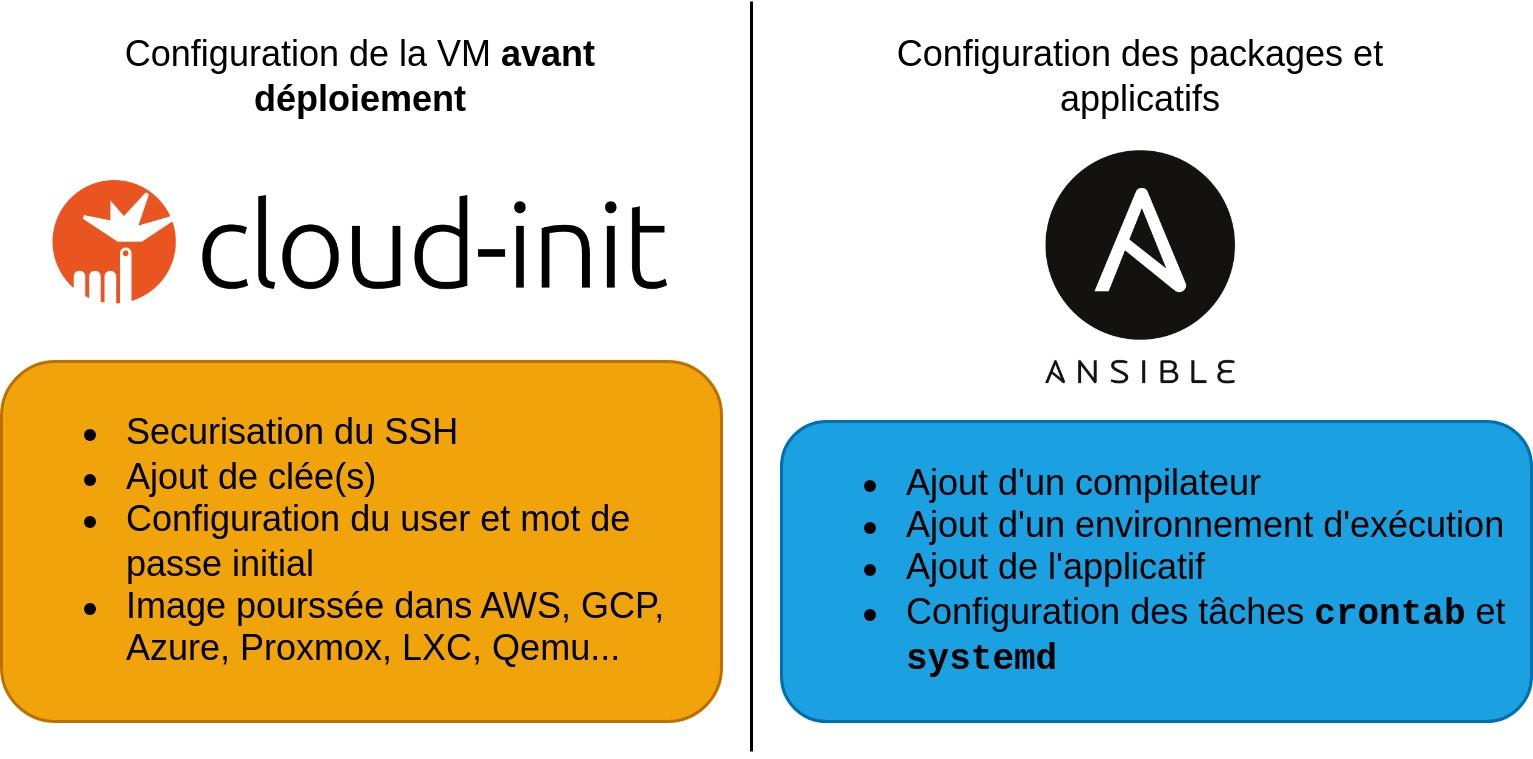
\includegraphics[width=12cm]{image/cloud-init-vs-ansible}
    \end{frame}


    \section{Préparation de la VM}\label{sec:prepare-vm}
    \begin{frame}{Configuration du SSH}{Sécurisation du SSH avec la cryptographie asymétrique}
        \begin{footnotesize}
            Pourquoi est-ce plus sécure d'utiliser une clé SSH plutôt qu'un mot de passe~?
            \bigbreak
            Quels algorithmes et taille de clé sont recommandés~?
            \pause
            \bigbreak
            Sur le site \url{https://jadaptive.com/ssh-key-management/the-benefits-of-ssh-key-authentication/} on trouve~:
            \begin{columns}
                \begin{column}{0.6\textwidth}
                    \begin{itemize}
                        \item Le mot de passe doit être communiqué à chaque connexion, il est donc plus vulnérable à une interception/sniffing/MITHM~.
                        La clé privée reste sur le client, elle n'est pas communiquée.
                        \item La clé SSH est plus complexe à deviner qu'un mot de passe.
                        \item On peut automatiser des taches depuis la machine cliente avec la clé SSH~.
                    \end{itemize}
                \end{column}
                \begin{column}{0.4\textwidth}
                    \centering
                    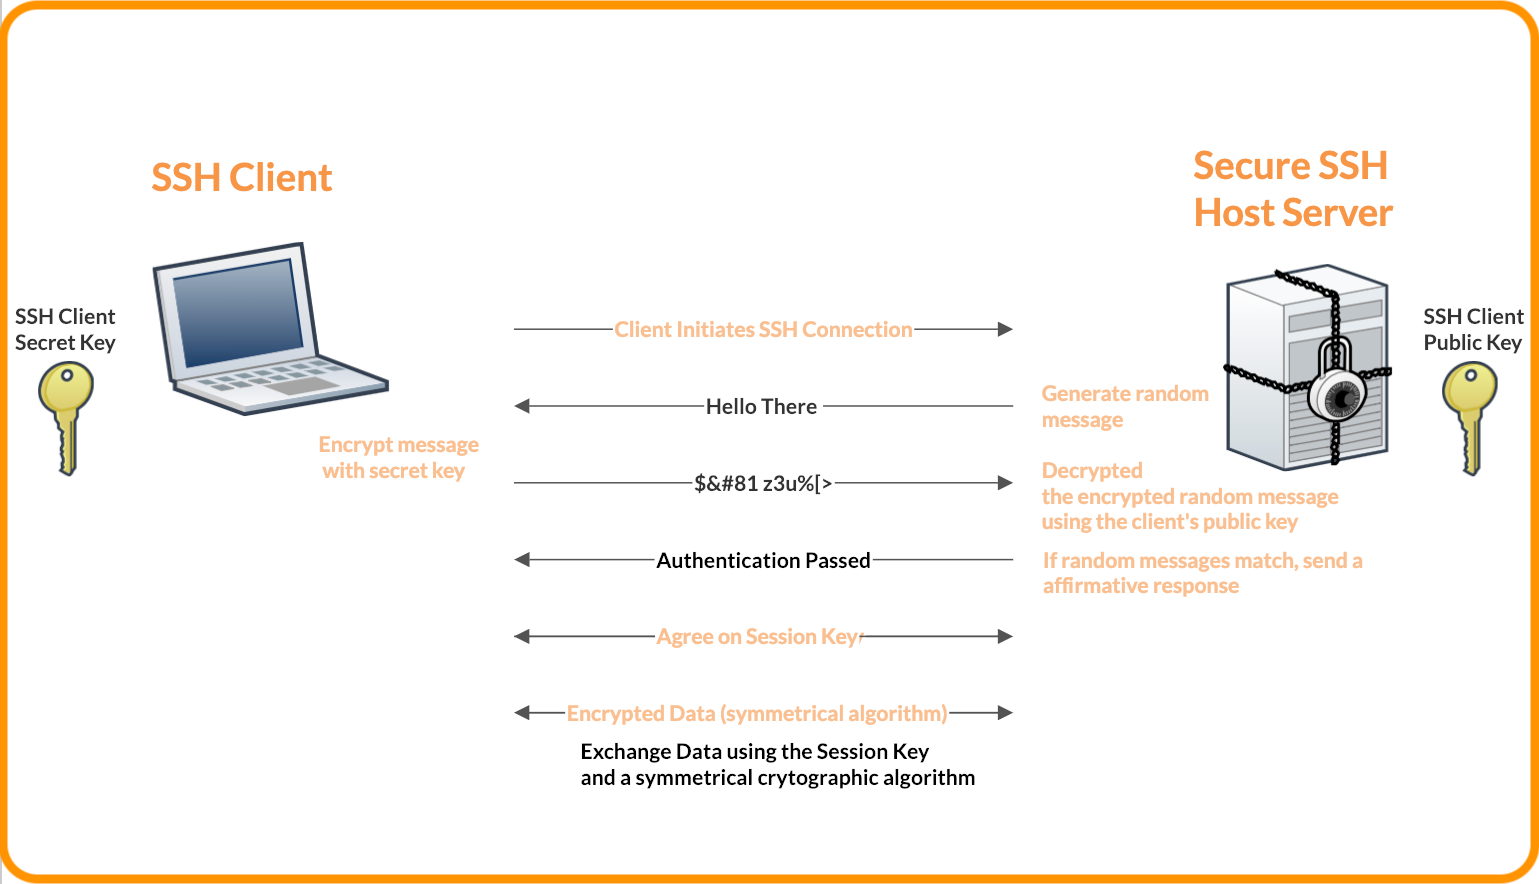
\includegraphics[width=5cm]{image/ssh-key-diagram} \\ Foxpass\footnotemark \\
                \end{column}
            \end{columns}
            \footnotetext{Learn SSH Keys in Minutes, \url{https://www.foxpass.com/blog/learn-ssh-keys-in-minutes/}}
        \end{footnotesize}
    \end{frame}

    \begin{frame}[fragile]{Configurer le SSH}{Une des solutions (commande à exécuter sur la VM)}
        Commande pour configurer la VM~:
        \begin{lstlisting}[language=bash][fragile]
# Configure SSH
sed -i '/PermitRootLogin/d' /etc/ssh/sshd_config
echo "PermitRootLogin no" >> /etc/ssh/sshd_config
sed -i '/PasswordAuthentication/d' /etc/ssh/sshd_config
echo "PasswordAuthentication no" >> /etc/ssh/sshd_config
# Restart SSH with the new configuration
sudo systemctl restart sshd
# Create the .ssh directory and the authorized_keys file
mkdir -p ~/.ssh
touch ~/.ssh/authorized_keys
# Add the public key to the authorized_keys file
echo "ssh-rsa AAAAB3NzaC1yc2EAAAADAQABAAABgQDQ8z4... chrichri@localhost" >> ~/.ssh/authorized_keys
        \end{lstlisting}
        \begin{columns}
            \column{0.5\textwidth}
            Expliquer chaque commande.
            \column{0.5\textwidth}
            \begin{center}
                
\includegraphics[width=2cm]{image/funny-key}
            \end{center}
        \end{columns}
    \end{frame}

    \begin{frame}{Cloud-init\footnote{Cloud-init, The standard for customising cloud instances, \url{https://cloud-init.io/}}}
        Cloud-init est un outil qui permet de configurer une VM lors de son déploiement.
        \bigbreak
        Il est possible de configurer~:
        \begin{itemize}
            \item Le nom de la machine.
            \item Les utilisateurs.
            \item Les clés SSH.
            \item Les scripts à exécuter.
        \end{itemize}
        Il est compatible avec la plupart des hyperviseurs et \textit{cloud providers}.
        \bigbreak
        \centering
        
\includegraphics[width=10cm]{image/cloud-init}
    \end{frame}

    \begin{frame}{Cloud-init}{Déploiement d'une VM vierge sécurisée}
        Exercice \execcounterdispinc{}~:
        Avec Cloud-init dans un premier script Shell~:
        \begin{itemize}
            \item Restreindre l'accès à la VM au SSH avec une clé SSH, aucun mot de passe.
            \item Pas de root en SSH
            \item Créez un user pour un de vos camarades.
            \item Donner un Shell \lstinline{bash} par défaut.
        \end{itemize}
        Dans un second script Shell~:
        \begin{itemize}
            \item Lancer la VM
        \end{itemize}
        Utiliser des images cloud pour Qemu de chez Ubuntu ou Rocky Linux.
    \end{frame}


    \section{Ansible}\label{sec:ansible}

    \begin{frame}{Automatisation de la configuration avec Ansible}{Définition\footnote{Ansible Community Documentation, \url{https://docs.ansible.com/ansible/latest/getting_started/index.html}}}
        Ansible est un outil d'automatisation de la configuration des machines physiques ou virtuelles déjà existantes.
        Inutile pour les containers, car leur configuration a les mêmes capacités.
        Il permet de définir des \textquote{playbooks} qui décrivent une configuration à appliquer aux machines qui sont dans l'\textquote{inventory} .
        \bigbreak
        \centering
        
\includegraphics[width=3cm]{image/logo-ansible}
    \end{frame}

    \begin{frame}[fragile]{Automatisation de la configuration avec Ansible}{Exemple d'inventaire}
        Pour accéder à la VM créée précédemment dans Qemu, il faut définir un inventaire avec les données dont on aurait besoin pour y accéder en SSH~.
        \begin{lstlisting}[language=bash,basicstyle=\ttfamily\tiny]
$ ssh chrichri@localhost -p 5022 -v -i /home/chrichri/Documents/Campus-St-Michel-IT/production-deployment/virt-ubuntu
        \end{lstlisting}
        La commande ci-dessus, devient dans l'inventaire (on peut créer des variables)~:
        \begin{lstlisting}[language=bash,basicstyle=\ttfamily\tiny]
[gunicorn]
localhost:5022 ansible_ssh_private_key_file=/home/chrichri/Documents/Campus-St-Michel-IT/production-deployment/virt-ubuntu ansible_ssh_user=chrichri
        \end{lstlisting}
        On utilise le module \lstinline{ping} pour vérifier que l'accès SSH est correctement configuré.
        \begin{lstlisting}[language=bash,basicstyle=\ttfamily\tiny]
$ ansible gunicorn -m ping -i inventory.ini
localhost | SUCCESS => {
    "ansible_facts": {
        "discovered_interpreter_python": "/usr/bin/python3"
    },
    "changed": false,
    "ping": "pong"
}
        \end{lstlisting}
    \end{frame}

    \begin{frame}{Automatisation de la configuration avec Ansible}{Aucune installation côté client\emoji{heart}}
        Pourquoi Ansible n'a aucun client sur les machines de l'inventaire~?
        \bigbreak
        \centering
        
\includegraphics[width=5cm]{image/question-mark-on-a-blank-background}
        \bigbreak
        \pause
        \flushleft
        Avec le seul accès SSH, il exécute les commandes qu'il faut.
        Il est agnostique à l'OS~!
    \end{frame}

    \begin{frame}[fragile]{Automatisation de la configuration avec Ansible}{Exemple de \textquote{playbook}}
        Qu'a-t-on installé sur un Ubuntu \textit{cloud image} comme package(s) pour pouvoir exécuter l'application gunicorn Hello World~?
        \pause
        % With apt, packages python3-gunicorn
        \begin{lstlisting}[language=bash]
sudo apt-get install python3-gunicorn
        \end{lstlisting}
        Commande qui devient dans un playbook Ansible \lstinline{gunicorn.yml}~:
        \begin{lstlisting}
---
- name: gunicorn
  hosts: gunicorn
  become: yes # Run as root
  tasks:
  - name: Install gunicorn
    apt:
      name: gunicorn # Le package à installer
      state: present
        \end{lstlisting}
        À lancer avec la commande~:
        \begin{lstlisting}[language=bash]
$ ansible-playbook -i inventory.ini gunicorn.yml
        \end{lstlisting}
    \end{frame}

    \begin{frame}[fragile]{Automatisation de la configuration avec Ansible}{Exemple de \textquote{playbook}}
        Le résultat de l'exécution du playbook \lstinline{gunicorn.yml}~:
        \begin{lstlisting}[language=bash]
$ ansible-playbook -i inventory.ini gunicorn.yml
...
localhost                  : ok=2    changed=1    unreachable=0    failed=0    skipped=0    rescued=0    ignored=0

$ ansible-playbook -i inventory.ini gunicorn.yml
...
localhost                  : ok=2    changed=0    unreachable=0    failed=0    skipped=0    rescued=0    ignored=0
        \end{lstlisting}
        À la première exécution, le package est installé, à la seconde il est déjà installé, aucun changement.
    \end{frame}

    \begin{frame}[fragile]{Automatisation de la configuration avec Ansible}{Commande pour exécuter un programme}
        Une fois les dépendances requises installées, on peut exécuter un programme avec le module \lstinline{shell}~.
        \bigbreak
        S’il faut copier un ou plusieurs fichiers, on peut utiliser le module \lstinline{copy}~.
        \bigbreak
        Par exemple~:
        \begin{lstlisting}
---
- hosts: gunicorn # Groupe de host de l'inventory
  vars:
  - EXEC_ABS_PATH: /home/chrichri/helloworld # Utilisé 2 fois donc dans une variable
...
  - name: Copy Application
    copy:
      src: /home/chrichri/Documents/Campus-St-Michel-IT/production-deployment/helloworld/build/helloworld # Le build de ma machine
      dest: "{{ EXEC_ABS_PATH }}"

  - name: Run Application
    shell: nohup {{ EXEC_ABS_PATH }} & # nohup pour exécuter en arrière plan
        \end{lstlisting}
    \end{frame}

    \begin{frame}{Automatisation de la configuration avec Ansible}{La Ansible Galaxy}
        Comme souvent, inutile de tout recoder.
        Ansible est modulaire grâce aux \textquote{roles} et aux \textquote{playbooks} qui sont eux-mêmes des modules\footnote{Roles, \url{https://docs.ansible.com/ansible/latest/playbook_guide/playbooks_reuse_roles.html}}.
        \bigbreak
        La communauté Ansible a packagé des modules et des playbooks pour les tâches les plus courantes\footnote{Ansible Galaxy, \url{https://galaxy.ansible.com/ui/}}.
        Ils sont disponibles sur la \href{https://galaxy.ansible.com/}{Ansible Galaxy}.
        Et peuvent être installés avec la commande \lstinline{ansible-galaxy install <module>}, commande issue du package \lstinline{ansible-core}.
    \end{frame}

    \begin{frame}{Automatisation de la configuration avec Ansible}{Ansible et Windows}
        Sur la machine hôte, on ne peut l'installer que depuis un WSL~.
        \begin{dangercolorbox}
            Si la machine cliente est un Windows, attention au package manager et aux séparateurs de chemin, voir \url{https://docs.ansible.com/ansible/latest/os_guide/windows_usage.html}.
        \end{dangercolorbox}
        \bigbreak
        \centering
        
\includegraphics[width=5cm]{image/broken-windows} \\ L'idéal reste quand même de ne pas utiliser Windows\ldots \\
    \end{frame}

    \begin{frame}{Automatisation de la configuration avec Ansible}{Exercice \execcounterdispinc{}}
        En utilisant la VM créée à l'exercice précédent, configurer un inventaire et un playbook pour installer un serveur MySQL.
        \bigbreak
        Vous pouvez vous aider du tutoriel de Digital Ocean \href{https://www.digitalocean.com/community/tutorials/how-to-import-and-export-databases-in-mysql-or-mariadb}{How To Import and Export Databases in MySQL or MariaDB} pour importer un jeu de test correspondant à un serveur DNS \url{https://gist.github.com/Habbie/5466890}.
        \bigbreak
        \centering
        
\includegraphics[width=6.5cm]{image/happy-dolphin}
    \end{frame}

    \begin{frame}{Automatisation de la configuration avec Ansible}{Exercice \execcounterdispinc{}}
        En utilisant la VM créée à l'exercice précédent, configurer un inventaire et un playbook pour installer l'application Spring Boot et la connecté à la base de donnée MySQL de l'autre exercice.
        \bigbreak
        Vous pouvez vous aider du \href{https://spring.io/guides/gs/spring-boot}{tutoriel officiel}.
        \bigbreak
        \centering
        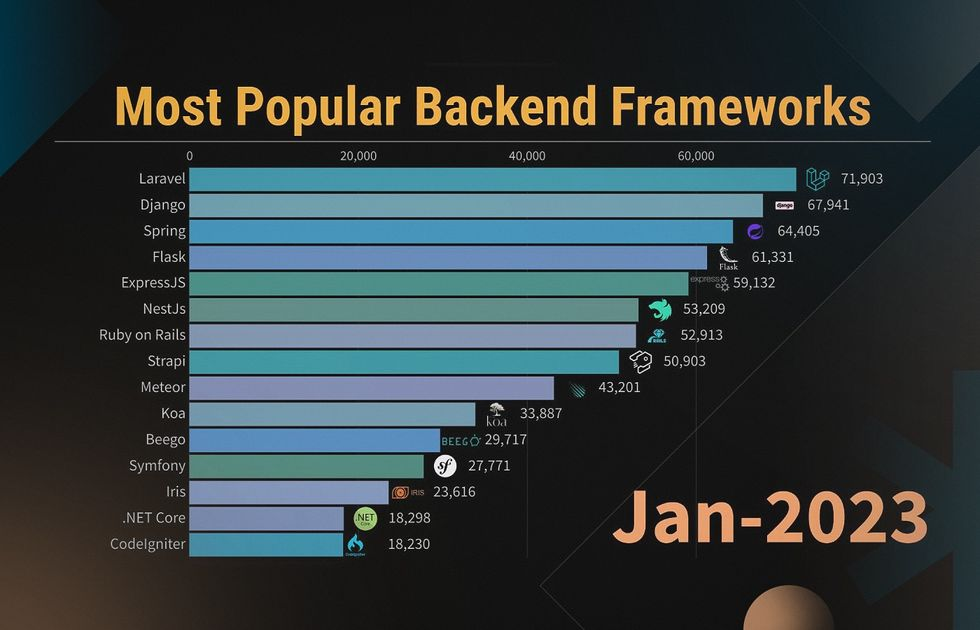
\includegraphics[width=8cm]{image/most-popular-backend}
    \end{frame}

    \begin{frame}{Automatisation de la configuration avec Ansible}{Solution à l'exercice précédent}
        De nombreuses solutions sont valides.
        Mais avec Java il est plus simple de profiter du \textquote{Write once, run anywhere}.
        \bigbreak
        Ce n'est donc pas obliger d'utiliser un système de build comme Maven ou Gradle sur la VM, Java suffit pour exécuter une JAR~.
        \bigbreak
        Une JAR (Java ARchive) est un exécutable qui contient toutes les classes zippées et qui se lance avec \lstinline{java -jar <JAR file>}.
        Il suffit donc d'installer Java sur la JVM~.
    \end{frame}

    \begin{frame}[fragile]{Automatisation de la configuration avec Ansible}{Solution à l'exercice précédent}
        Par exemple, une solution avec uniquement Java 17~:
        \begin{lstlisting}[basicstyle=\ttfamily\tiny]
---
- hosts: gunicorn
  vars:
  - JAR_DEST_PATH: /home/chrichri/helloworld-0.0.1-SNAPSHOT.jar
  become: yes
  tasks:
  - name: Update APT package index
    apt:
      update_cache: yes

  - name: Install Java 17
    apt:
      name: openjdk-17-jre-headless
      state: present

  - name: Copy Spring Boot Application
    copy:
      src: /home/chrichri/Documents/Campus-St-Michel-IT/production-deployment/helloworld/build/libs/helloworld-0.0.1-SNAPSHOT.jar
      dest: "{{ JAR_DEST_PATH }}"

  - name: Run Spring Boot Application
    shell: nohup java -jar {{ JAR_DEST_PATH }} &
        \end{lstlisting}
    \end{frame}


    \section{Scripting Python}\label{sec:scriptingpython}

    \subsection{Proxmox API}\label{subsec:proxmoxapi}

    \begin{frame}{Scripting Python}
        Pourquoi utiliser Python et non pas Shell~?
        \bigbreak
        \centering
        
\includegraphics[width=10cm]{image/python-vs-bash}
    \end{frame}

    \begin{frame}{Scripting Python}
        Quel protocole est principalement utilisé pour les API web~?

        Quelle(s) librairie(s) est disponible dans Shell a pour communiquer avec ce protocole~?
        \bigbreak
        \centering
        
\includegraphics[width=5cm]{image/baby-shell}
        \pause
        \begin{itemize}
            \item Pas de package manager~!
            On ne peut pas publier un client prêt à l'emploi~!
            \item Pas de libraire pour les requêtes à part Curl.
            \item Pas d'IDE utilisant des fonctionnalités modernes (autocomplétion, \textit{etc})
            \item \ldots
        \end{itemize}
    \end{frame}

    \begin{frame}{Scripting Python sur Proxmox}{Développement d’un script de gestion de VM avec Proxmox API}
        \footnotesize
        \begin{columns}
            \column{0.8\textwidth}
            La documentation de l'API de Proxmox est disponible sur \url{https://pve.proxmox.com/pve-docs/api-viewer/}.
            \begin{itemize}
                \item Créer une VM sur le Proxmox, ou utiliser celle de l'exercice précédent.
                \item Pour s'authentifier~:
                \begin{itemize}
                    \footnotesize
                    \item Option 1, aller à \textit{Permissions} / \textit{API Tokens} / \textit{Add} pour créer un token.
                    \item Option 2, demander un \textit{access ticket} avec \lstinline{POST /api2/json/access/ticket}, avec les champs \lstinline{username}, \lstinline{password}.
                    Utiliser le \textit{ticket} pour s'authentifier à tous les autres endpoints.
                    En ajoutant dans le cookie la valeur PVEAuthCookie et dans le header la valeur CSRFPreventionToken retournée précédemment par le \lstinline{POST /api2/json/access/ticket}.
                \end{itemize}
                \item (Optionnel) Installer Postman pour tester les requêtes et les extraire en Python avec la libraire \href{https://fr.python-requests.org/en/latest/}{requests} une fois validée.
                \item Toutes les fonctionnalités de l'API devraient maintenant être accessibles.
            \end{itemize}
            \column{0.2\textwidth}
            \centering
            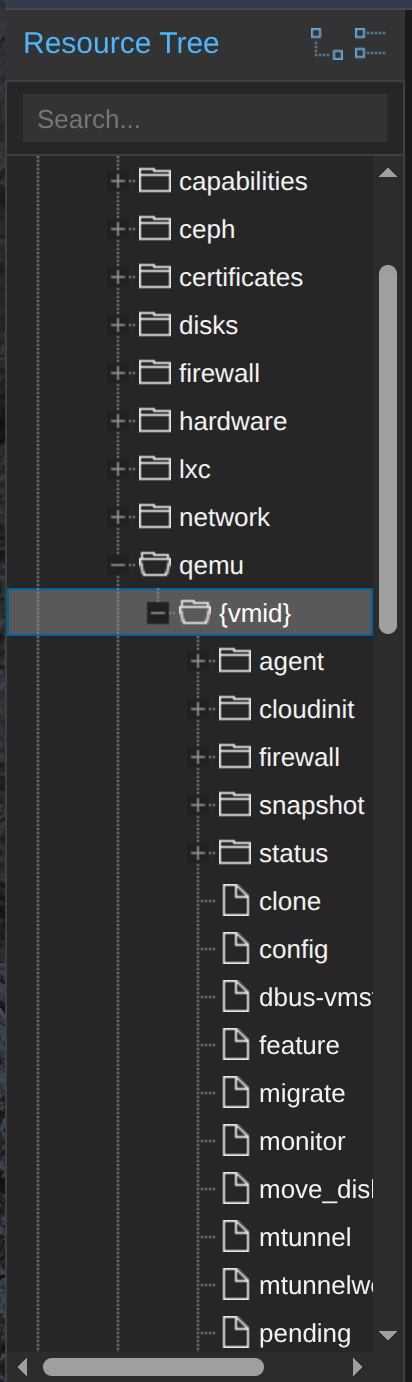
\includegraphics[width=2cm]{image/pve-api-viewer}
        \end{columns}
    \end{frame}

    \begin{frame}{Scripting Python sur Proxmox}{Exercice \execcounterdispinc{}, lecture de la documentation}
        Trouver les endpoints~:
        \begin{itemize}
            \item De création d'une VM.
            \item De création d'un conteneur LXC.
        \end{itemize}
        \bigbreak
        \centering
        
\includegraphics[width=5cm]{image/girl-rtfm.png}
    \end{frame}

    \begin{frame}{Scripting Python sur Proxmox}{Exercice \execcounterdispinc{}, développer un script Python avec CLI de management des VM}
        Mettez vous dans la peau d'un administrateur système de datacenter.
        Il vous est demandé de moduler la capacité du SI en fonction de la charge.
        Dans le but de répondre à cette demande, vous devez écrire un script Python qui~:
        \begin{itemize}
            \item N'a qu'une dépendance distante, le package \lstinline{requests}.
            \item Utilise les modules \lstinline{argparse} et \lstinline{logging} de la standard libray.
            \item Les logs doivent être dans un fichier CSV et compatible avec un viewer.
            \item La CLI a pour les arguments correspondants à ces fonctionnalités~:
            \begin{itemize}
                \item Arrêter une VM identifiée par son ID.
                \item Mettre en veille une VM identifiée par son ID.
                \item Sortir de la veille une VM identifiée par son ID.
                \item Démarrer de la veille une VM identifiée par son ID.
            \end{itemize}
            \item Vérifier le statut de la VM avant chaque action.
            Par exemple pour ne pas démarrer une VM qui tourne.
            \item Logger toutes les informations pertinentes.
        \end{itemize}
    \end{frame}

    \begin{frame}{Scripting Python sur Proxmox}{Exercice \execcounterdispinc{}, développer un script Python avec CLI de management des containers LXC}
        Mettez vous dans la peau d'un administrateur système de datacenter.
        Il vous est demandé de moduler la capacité du SI en fonction de la charge.
        Dans le but de répondre à cette demande, vous devez écrire un script Python qui~:
        \begin{itemize}
            \item N'a qu'une dépendance distante, le package \lstinline{requests}.
            \item Utilise les modules \lstinline{argparse} et \lstinline{logging} de la standard libray.
            \item Les logs doivent être dans un fichier CSV et compatible avec un viewer.
            \item La CLI a pour les arguments correspondants à ces fonctionnalités~:
            \begin{itemize}
                \item Créer un container LXC identifié par son ID.
                \item Démarrer un container LXC identifié par son ID.
                \item Stopper un container LXC identifié par son ID.
            \end{itemize}
            \item Vérifier le statut du container avant chaque action.
            Par exemple pour ne pas démarrer un container qui tourne déjà.
            \item Logger toutes les informations pertinentes.
        \end{itemize}
    \end{frame}

    \begin{frame}{Scripting Python sur Proxmox}{Les clients sont plus souvent à intégrer seulement, plus qu'à développer}
        Ces exercices permettent de se familiariser avec Python mais il existe déjà des clients plus ou moins officiels de l'API Proxmox dans de nombreux langages\footnote{API Client Libraries, \url{https://pve.proxmox.com/wiki/Proxmox_VE_API}}~:
        \begin{itemize}
            \item Python
            \item Java
            \item Go
            \item \ldots
        \end{itemize}
        \bigbreak
        Les clouds providers (Azure, AWS, OVH) publient également des clients Python de leurs API.
        Mais nous on a Proxmox \emoji{flexed-biceps}\ldots
    \end{frame}


    \section{Licence CC}\label{sec:licence}

    \begin{frame}{Licence}{Licence Creative Commons}
        Support de cours sous licence Creative Commons BY-NC-ND~.
        \bigbreak
        Vous pouvez donc, partager, copier, distribuer le document.
        \bigbreak
        Attribution requise à PapIT SASU - Pas d’utilisation commerciale - Pas de modification
        \bigbreak
        \centering
        
\includegraphics[width=5cm]{image/by-nc-nd-logo}
    \end{frame}
\end{document}
